\documentclass[8pt,notitlepage]{report}
\usepackage[utf8]{inputenc}
\usepackage[italian]{babel}
\usepackage{amsmath}
\usepackage{amsfonts}
\usepackage{amssymb}
\usepackage{makeidx}
\usepackage{graphicx}
\usepackage{hyperref}
\usepackage{float}
\usepackage{titling}
\usepackage{lipsum}
\usepackage[top=1in, bottom=1.25in, left=1.25in, right=1.25in]{geometry}
\usepackage[justification=justified, format=plain]{caption}
\usepackage[ruled]{algorithm2e}

\title{PeterPen}
\author{Dario Montagnini, Antonio Musolino, \\Manuel Prandini, Giovanni Varricchione}
\date{}

\graphicspath{ {images/} }

\begin{document}


\twocolumn
[
	\begin{@twocolumnfalse}
	\maketitle
	\begin{abstract}
		Lo scopo che ci siamo posti con questo progetto è stato la creazione di una penna che permettesse il riconoscimento biometrico di un utente tramite la sua scrittura. A tal fine, è  stata progettata e realizzata una penna che permettesse la cattura dei dati di scrittura degli utenti, inviandoli ad un server tramite una connessione Wi-Fi. La penna è stata realizzata con chip economici e la scocca tramite una stampante 3D. Sono stati implementati due diversi modelli per il riconoscimento biometrico, uno basato su un algoritmo di deep learning ed uno su distanze fra segnali. Sul dataset disponibile sono state osservate buone performance da entrambi i modelli, con risultati molto interessanti soprattutto per il modello di deep learning.
	\end{abstract}
  	\end{@twocolumnfalse}
]

\subsection*{Scrittura}
	La scrittura è uno dei tanti tratti che può essere usato in un sistema biometrico. È categorizzato come un tratto biometrico \textit{comportamentale}, in quanto è basato su un'azione appresa dall'utente, oltre al suo stato umorale nel momento della cattura dei dati (altri esempi di questi tratti sono il modo in cui si cammina e la battitura dei tasti). Generalmente, ha una bassa \textit{accuracy} ma un'elevata \textit{acceptability}.  \\
	Il tratto è principalmente influenzato da caratteristiche quali la calligrafia, la pressione esercitata e l'inclinazione della penna durante la scrittura.
\subsection*{Stato dell'arte}
	Tipicamente i sistemi di riconoscimento della scrittura si basano sul riconoscimento della firma dell'utente (ad esempio Karouni et al. \cite{Karouni15}). Tali sistemi sono anche detti di "\textit{signature recognition}", l'idea alla base di quest'approccio è che la firma varia notevolmente da individuo a individuo e quindi può essere sfruttata come tratto identificativo. Naturalmente, esistono anche sistemi che permettono il riconoscimento utilizzando qualsiasi parola, in questo caso si parla di "\textit{handwriting recognition}". Mentre i primi sono vulnerabili ad attacchi di \textit{spoofing}, i secondi sono più resistenti ma potrebbero avere performance più basse. \\
	Ci sono due approcci principali al riconoscimento della scrittura: il primo, detto "\textit{statico}" o "\textit{off-line}", si basa su tecniche di \textit{image processing}. La firma viene catturata e poi trasformata in un'immagine, che successivamente sarà analizzata dal modello (esempi sono Sharif et al.\cite{Sharif18} e Souza V., Oliveira A. e Sabourin R. \cite{Souza18}). Il secondo approccio, detto "\textit{dinamico}" o "\textit{on-line}", si basa invece sui segnali che vengono catturati tramite dei sensori posti su una penna. Tipici segnali analizzati sono la pressione, l'accelerazione e la rotazione, in quanto caratterizzano la scrittura. In genere, quest'ultimi sono più performanti rispetto ai primi. \\
	Un approccio dinamico molto simile a quello che verrà presentato è stato proposto con la BioPen da De Marsico M., Ponzi F., Scozzafava F. e Tortora G. \cite{DeMarsico18}, tuttavia vi sono delle differenze nei modelli proposti. Innanzitutto, nella PeterPen il modulo di Machine Learning usa le LSTM, mentre nella BioPen le SVM. La pressione, inoltre, è usata in modi diversi: mentre nella BioPen veniva misurata la pressione posta dall'utente nella presa della penna, nella PeterPen viene misurata la pressione esercitata sulla punta durante la scrittura. Questo ci ha permesso anche di automatizzare il processo di raccolta dei dati, considerando solo i periodi in cui la pressione misurata superava una certa threshold. Chiaramente questi due approcci all'utilizzo della pressione hanno anche ripercussioni differenti nel riconoscimento dell'utente. 

	
\chapter{Architettura del Sistema}
	\begin{figure}[H]
		\begin{center}
			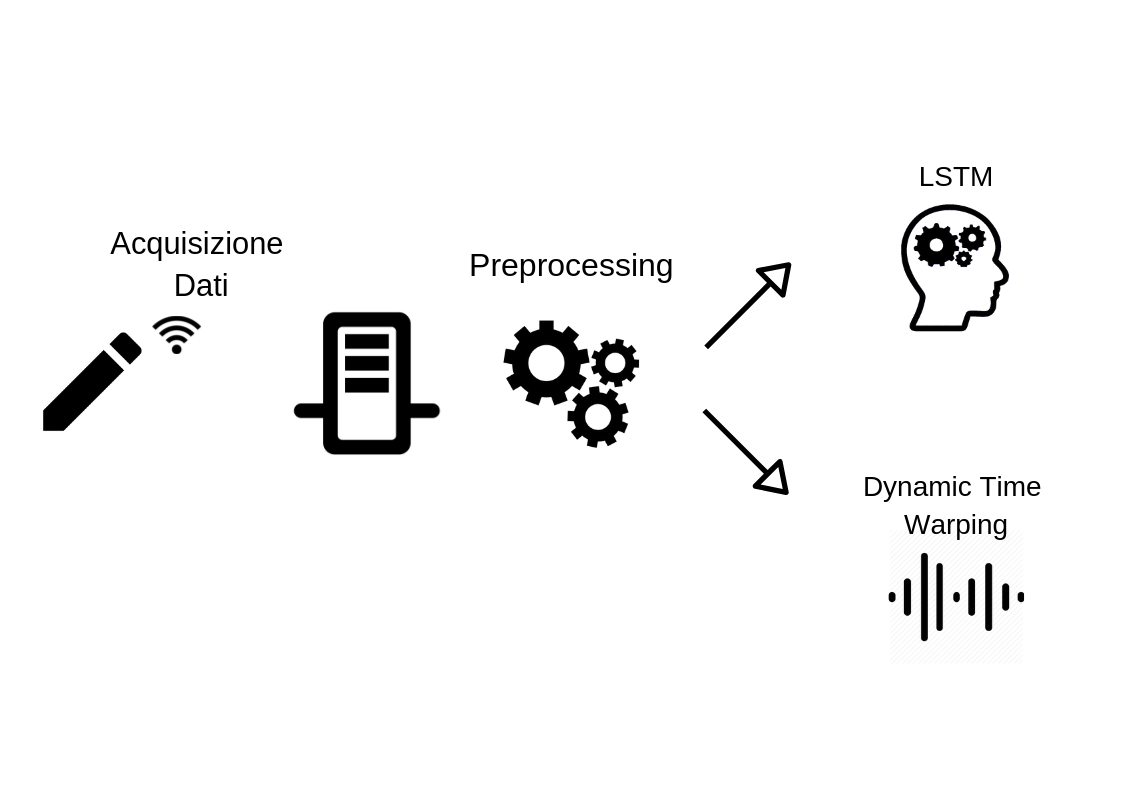
\includegraphics[scale=.25]{architettura}
			\caption{Schema dell'architettura}
		\end{center}
	\end{figure}		
	L'architettura del sistema è formata da 4 componenti: la penna, un server per l'acquisizione dei dati, e i moduli di \textit{preprocessing} dei dati e di classificazione. La penna raccoglie i dati tramite i sensori e li invia al server attraverso il modulo Wi-Fi del chip. I dati vengono salvati in appositi file JSON sul server (ad ogni utilizzo della penna è associato un file diverso) e possono essere quindi usati dal modulo di \textit{preprocessing}. Quest'ultimo si occupa principalmente di normalizzare i dati, in modo da renderli utilizzabili dai modelli di classificazione. Un modulo di classificazione è composto da una rete neurale che utilizza delle LSTM, mentre l'altro è basato sull'algoritmo \textit{Dynamic Time Warping}.

	\section{PeterPen}
		La penna è composta dal seguente hardware:
		\begin{itemize}
			\setlength\itemsep{.1em}
			\item un chip NODE MCU ESP8266;
			\item un accelerometro;
			\item un giroscopio;
			\item un sensore di pressione;
			\item un LED verde;
			\item un condensatore;
			\item due resistenze;
			\item una batteria da 9V;
			\item un involucro realizzato in PLA.
		\end{itemize}
		L'ESP8266, il chip principale della penna, è formato da un micro-controllore e da un modulo Wi-Fi utilizzato per la comunicazione con il server. A questo sono collegati accelerometro e giroscopio (contenuti all'interno di un unico chip), il sensore di pressione e il LED. \\
		Il sensore di pressione misura la forza applicata sulla punta della penna grazie all'ausilio di una molla. Subito dopo il sensore di pressione è posizionato il chip dell'accelerometro e del giroscopio e, dopo questo, si trova il microcontrollore. \\
		
		\begin{figure}[H]
			\label{figure:circuito}
			\begin{center}
				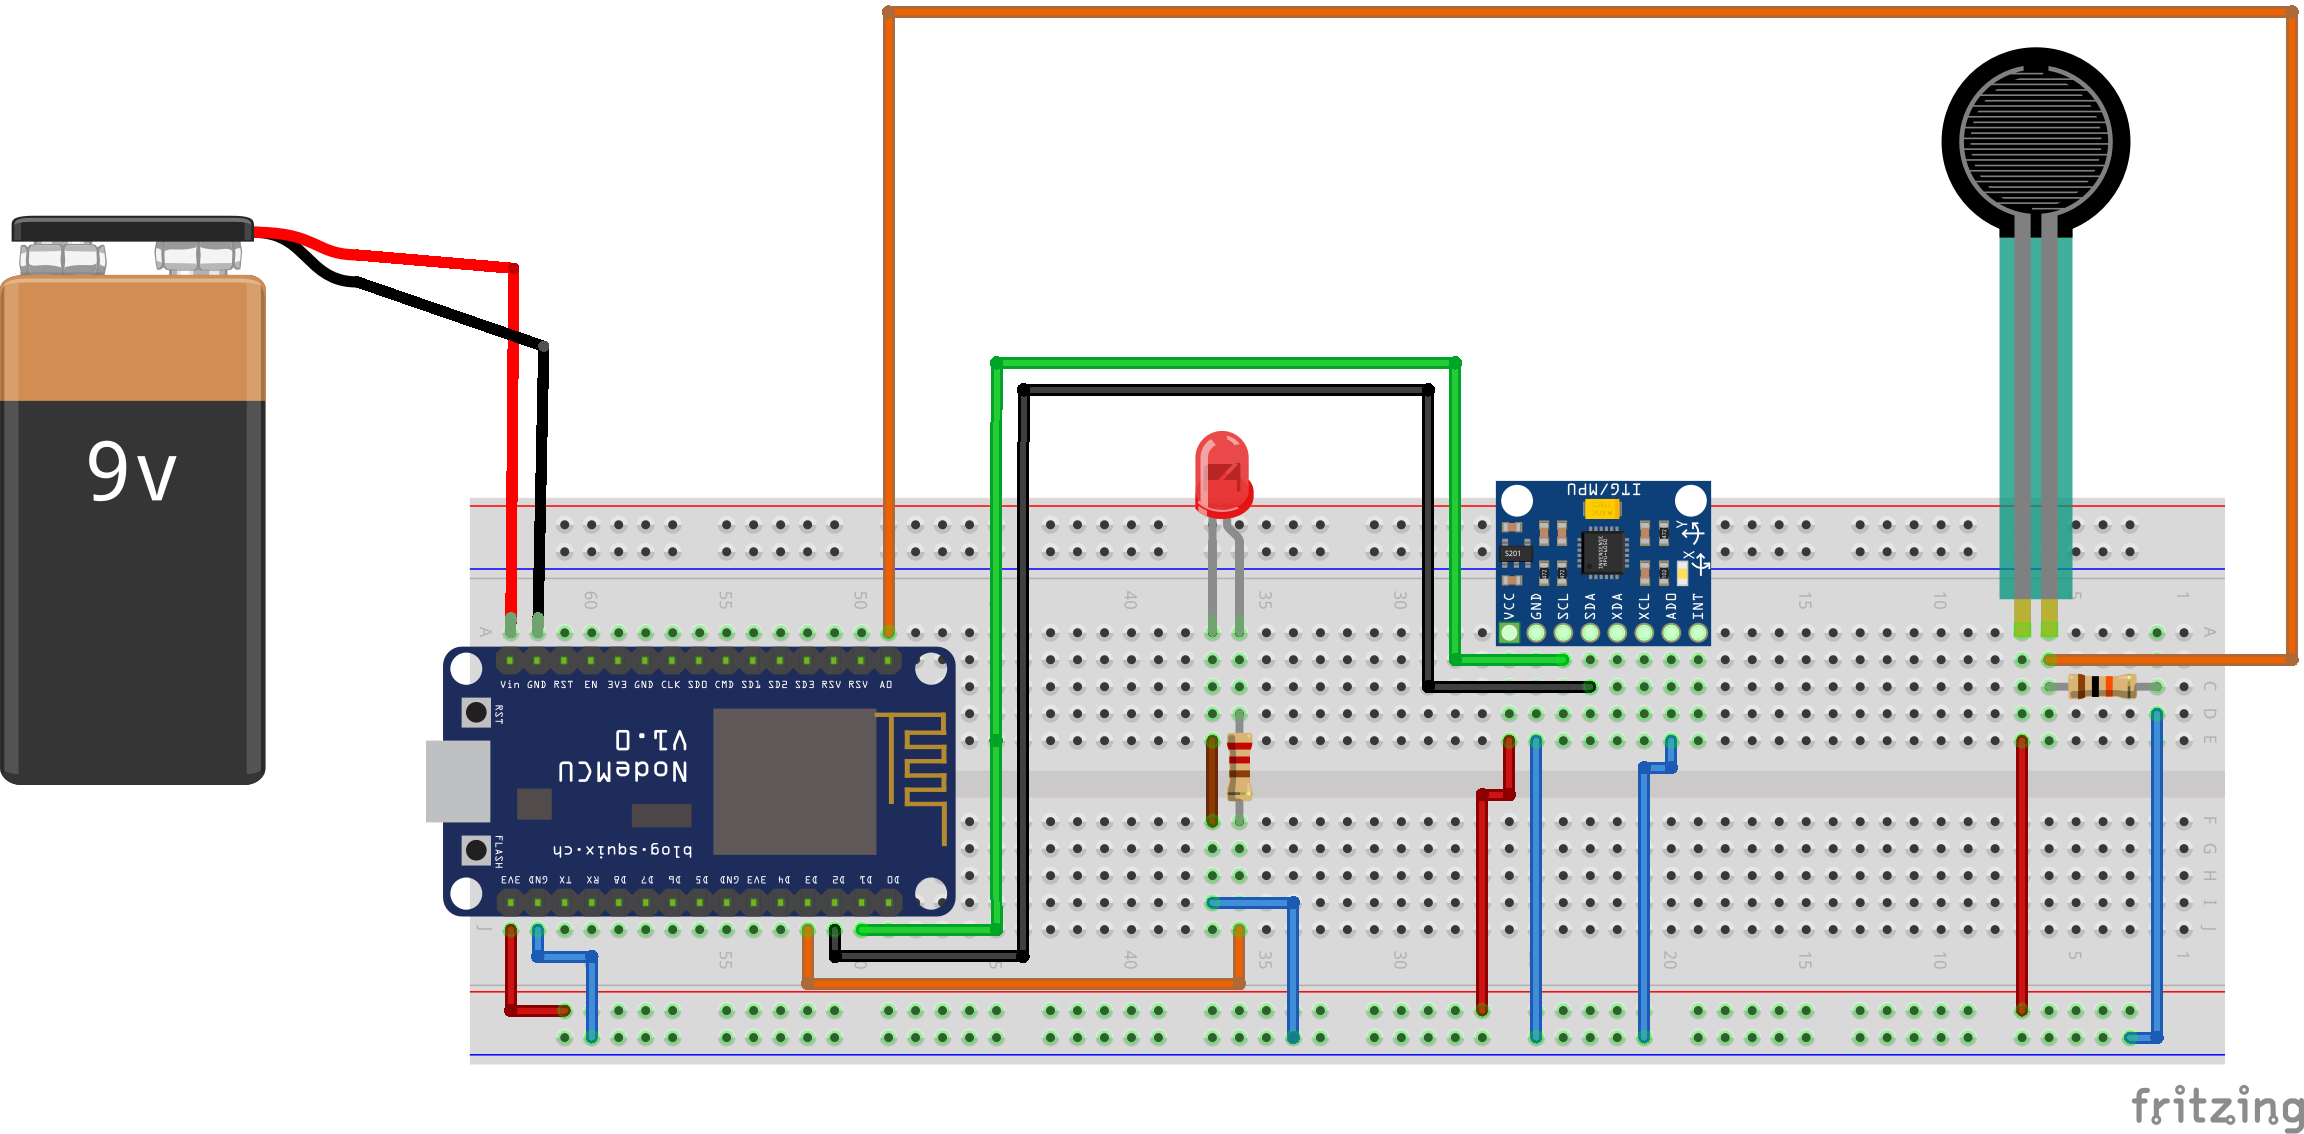
\includegraphics[scale=.35]{circuito}
				\caption{Circuito della PeterPen}
			\end{center}
		\end{figure}

		\begin{figure}[H]
			\begin{center}
				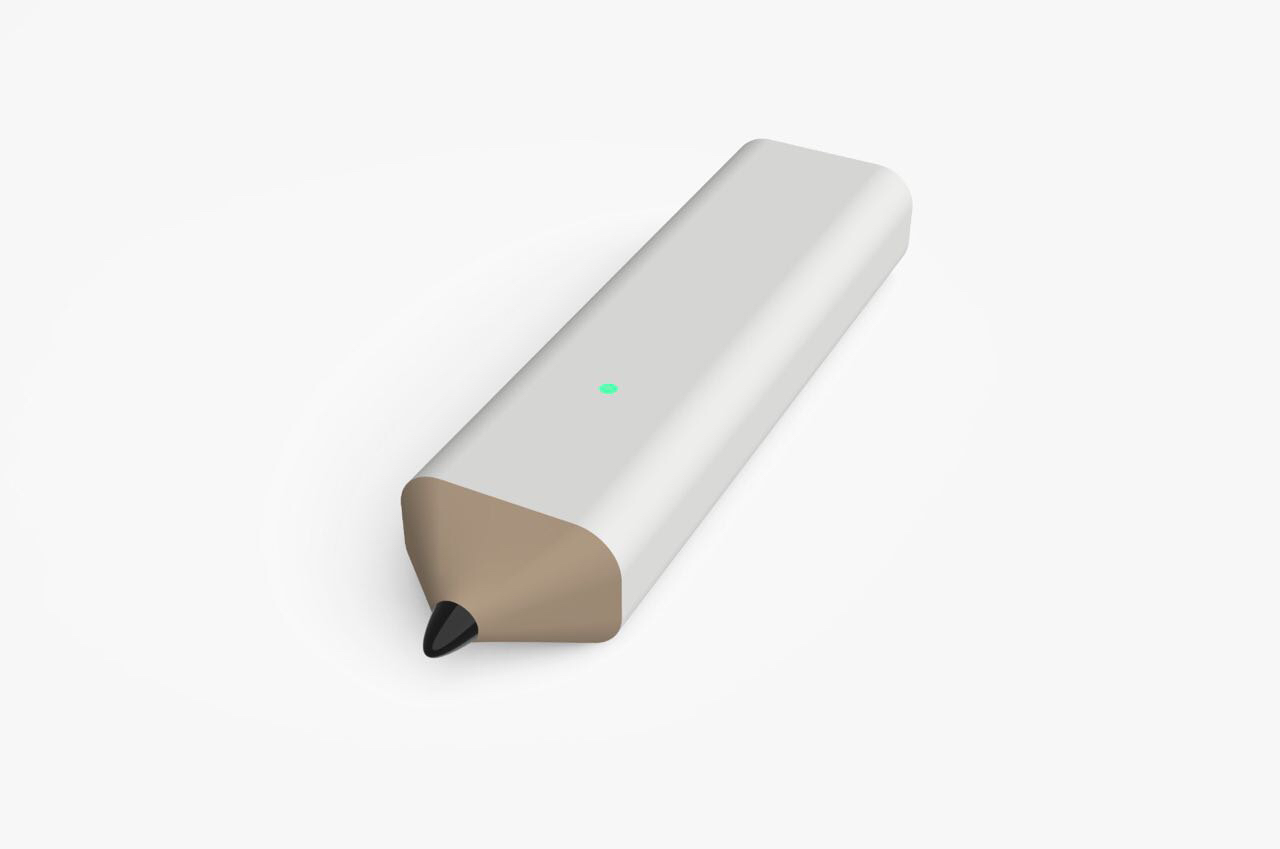
\includegraphics[scale=.1]{design}
				\caption{Design della PeterPen, si ringraziano Cristian Cianfarani e Tiziano Grossi}
			\end{center}
		\end{figure}		
		
		\begin{figure}[H]
			\begin{center}
				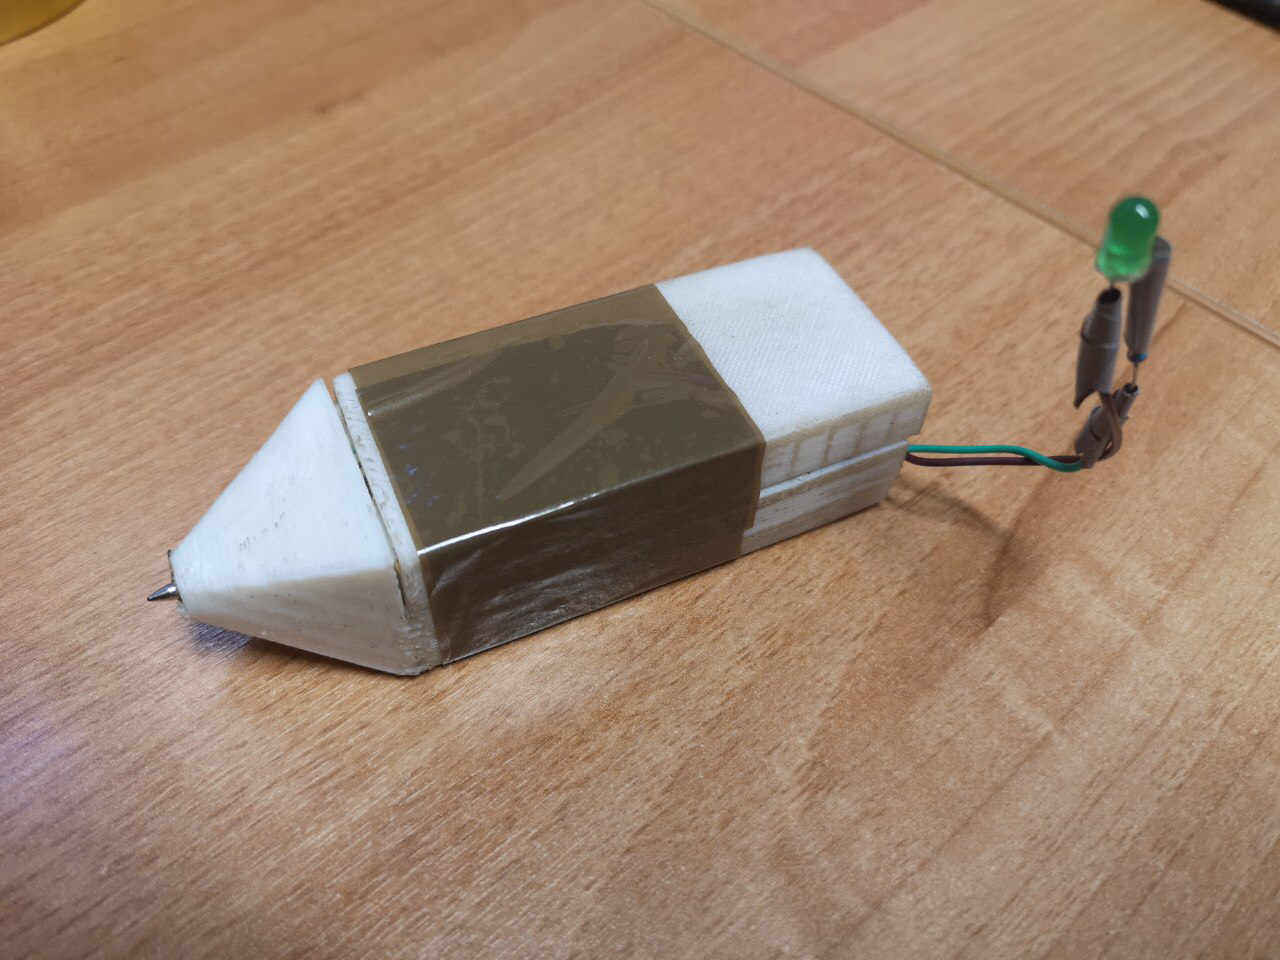
\includegraphics[scale=.105]{peterpen}
				\caption{PeterPen realizzata}
			\end{center}
		\end{figure}

		
		\subsection{Protocollo di acquisizione}
			È stato ideato un protocollo per semplificare l'acquisizione e l'invio dei dati. All'accensione della penna (che può essere alimentata o tramite un cavo USB o tramite batteria, usandone o una da 9V, come in \hyperref[figure:circuito]{figura}, o una da 3.3V o 3.6V, alimentandola però tramite il pin 3v3) il LED lampeggia durante la connessione alla rete e al server, o in caso di errore. Una volta connessa, il LED smette di lampeggiare e rimane acceso, questo indica all'utente che può iniziare a scrivere. Durante la scrittura la luce rimane spenta e, se non viene rilevata alcuna pressione per più di 2 secondi, si riaccende indicando la fine della scrittura della parola precedente e l'invio dei dati. È stato inoltre impostato come tempo massimo di scrittura 10 secondi, nel caso in cui l'utente superi tale limite il LED comincerà a lampeggiare, per segnalare l'errore e nessun dato sarà inviato.
		
		\subsection{Codice sorgente della penna}
			Il microcontrollore ESP8266 è programmato con un linguaggio derivato dal C, lo stesso che viene usato nella programmazione dei chip Arduino. Tale linguaggio richiede necessariamente l'implementazione di due funzioni in ogni programma. \\
			La prima, \verb|void setup()|, è eseguita un'unica volta all'inizio dell'esecuzione, ed è utilizzata per inizializzare le variabili. La seconda, \verb|void loop()|, rappresenta il kernel del programma ed è eseguito continuamente finché il chip è attivo, nel nostro caso l'esecuzione avviene ogni 10 millisecondi. \\
			Nel nostro caso, nella funzione \verb|setup|, vengono invocate altre due funzioni: \verb|mpu6050Begin| che inizializza il chip del giroscopio e dell'accelerometro e \verb|connect| che si occupa di effettuare la connessione al server. La funzione \verb|loop| ad ogni iterazione legge il valore della pressione e, in base allo stato (che è uno fra \verb|READY|, \verb|WRITING| e \verb|ERROR|) e alla variabile \verb|counter_writing| si comporterà diversamente. \\ Se la pressione registrata è sufficiente e lo stato è \verb|READY|, allora la penna passa allo stato \verb|WRITING|, acquisisce i dati e inizializza il contatore \\ \verb|counter_writing|. Invece, se la pressione è maggiore di un certo threshold, lo stato è \verb|WRITING| e sono passati meno di 10 secondi dall'inizio della scrittura allora acquisiti i dati dai sensori; nel caso in cui sono passati 10 o più secondi allora la penna si sposterà nello stato \verb|ERROR|. Infine, se lo stato è \verb|WRITING| e sono passati almeno 2 secondi da quando non si rileva abbastanza pressione, vengono inviati i dati al server e viene impostato lo stato \verb|READY|. 
			
	\section{Server}
		Il server è programmato in Node.js, in ascolto sulla porta 8080 mediante una socket TCP. Ad ogni nuova connessione crea un nuovo file JSON all'interno della quale andrà a salvare tutti i dati ricevuti dalla PeterPen, effettuandone precedentemente il parsing. Nel momento in cui la sessione viene chiusa, il server si occupa di gestire la chiusura del file relativo alla stessa.
		
		\subsection{File JSON}
			Il file contiene un array di parole, ed ogni parola è composta da una sequenza di lunghezza variabile (ma lunga al più 1000) di vettori composti dalle 7 feature. \\
			Le feature raccolte sono le seguenti:
			\begin{enumerate}
				\setlength\itemsep{.1em}
				\item componenti $ x, y $ e $ z $ dell'accelerometro;
				\item componenti $ x, y $ e $ z $ del giroscopio;
				\item valore della pressione.
			\end{enumerate}


\chapter{Classificazione}

	\section{Preprocessing}
		Nella fase di preprocessing i dati sono stati normalizzati, effettuando il rescaling delle singole feature, ed è stato aggiunto del padding per rendere i vettori delle singole parole lunghi esattamente 1000. Il padding è stato eseguito per entrambi i modelli, mentre il rescaling solo per il DTW (poiché peggiorava le prestazioni dell'LSTM, abbiamo deciso di non usare i dati scalati in quel caso). \\
		
		\subsection{Normalizzazione}
			I  dati sono stati normalizzati utilizzando la funzione di rescaling: 
			\[ rescaling(x) = \frac{x - min}{max - min} \]
			A tal fine, come valori minimi e massimi abbiamo usato:
			\begin{itemize}
				\setlength\itemsep{.01em}
				\item $ \pm 250 $ per i dati dell'accelerometro;
				\item $ \pm 2 $ per i dati del giroscopio;
				\item $ 0 $ e $ 1024 $ per i dati del sensore di pressione.
			\end{itemize}
	
	\section{DTW}
		L'algoritmo DTW (\textit{Dynamic Time Warping}) è un algoritmo di programmazione dinamica che permette di misurare la similarità fra due sequenze temporali; la particolarità dell'algoritmo è che riconosce anche sequenze che variano in velocità. Nel nostro caso, un esempio immediato è dato da un individuo che, scrivendo la stessa parola, impiega meno tempo a scriverla nel primo caso che nel secondo. \\
		Il DTW calcola l'\textit{optimal matching} fra due sequenze con le seguenti regole e restrizioni:
		\begin{enumerate}
			\item ogni elemento di una sequenza deve essere associato ad almeno un elemento dell'altra (ma non necessariamente ad uno solo);
			\item il primo elemento della prima sequenza deve essere associato al primo della seconda;
			\item l'ultimo elemento della prima sequenza deve essere associato all'ultimo della seconda;
			\item il matching deve essere \textit{monotono} e \textit{crescente}, ossia, dati due indici della prima sequenza $ i, j $ tali che $ i < j $, allora non possono esistere due indici della sequenza $ k, q $ tali che $ k < q $, $ q $ è stato associato a $ i $ e $ k $ è stato associato a $ j $.
		\end{enumerate}
		Ad ogni \textit{matching} è associato un costo (tipicamente la somma delle distanze euclidee fra ogni coppia di indici associati, che abbiamo usato nella nostra implementazione), e quello ottimale è quello il cui costo è minimo.
		\begin{algorithm}[h]
			\SetAlgoLined
			\caption{DTW}
			\KwData{$ s_1: [1 \dots n], s_2: [1 \dots m] $}
			\KwResult{distanza minima fra le due sequenze}
				$ \text{DTW } :=  [0 \dots n, 0 \dots m] $ \\
				\For{i := 0 to n }{
					$ \text{DTW}[i, 0] $ := $ \infty $
				}
				\For{j := 0 to m }{
					$ \text{DTW}[0, j] $ := $ \infty $
				}
				$ \text{DTW}[0, 0] = 0 $ \\
				\For{i := 1 to n}{
					\For{j := 1 to m}{
						$ \text{cost } := d(s_1[i], s_2[j]) $ \\
						$ \text{DTW}[i, j] = \text{cost } + $ \\ $  \min(\text{DTW}[i - 1, j], $ \\ $ \text{DTW}[i, j - 1], \text{DTW}[i - 1, j - 1]) $						
					}
				}
				$ \textit{return } \text{DTW}[n, m] $
		\end{algorithm}
		
		L'algoritmo costruisce una matrice $ n \times m $, dove $ n $ ed $ m $ sono rispettivamente le lunghezze delle due sequenze, e riempie ogni cella $ i, j $ della matrice con la distanza minima per raggiungerla dalla cella $ [0, 0] $; l'output è dato quindi dal valore nella cella $ [n, m] $. \\
		Per l'implementazione di quest'algoritmo abbiamo usato la libreria disponibile su GitHub al seguente link: \href{https://github.com/pierre-rouanet/dtw}{github.com/pierre-rouanet/dtw}.
		

	\section{LSTM}
		Le LSTM (\textit{Long Short Term Memory}) sono un'architettura di RNN (\textit{Recurrent Neural Network}). Le RNN sono una classe di reti neurali in cui l'output ad un certo istante $ t $ è passato anche in input alla rete nell'istante successivo $ t + 1 $. Uno degli strati al suo interno è utilizzato come memoria, e questo permette alla rete di riconoscere sequenze di valori, utilizzando sia il valore di input all'istante $ t $ sia lo stato interno (che è ottenuto dalla sequenza di input fino all'istante $ t - 1 $). 
		
		\begin{figure}[H]
			\begin{center}
				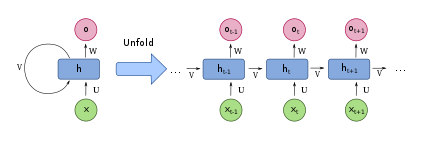
\includegraphics[scale=.55]{rnn}
				\caption{Una RNN "srotolata"}
			\end{center}
		\end{figure}
		
		Il problema delle RNN tuttavia è che, utilizzando la \textit{back-propagation} per effettuare l'aggiornamento dei pesi, i gradienti possono svanire fino a raggiungere $ 0 $ o esplodere. Nel primo caso, possiamo immaginarci che la RNN si scordi le informazioni che ha visto "troppo tempo fa". \\
		Per risolvere il primo problema, le LSTM permettono ai gradienti di non essere modificati quando vengono passati in input alla rete nell'istante successivo. In particolare, la rete utilizza uno strato per decidere quanto "ricordare" una determinata informazione, moltiplicando il valore per un numero compreso fra $ 0 $ e $ 1 $ (si noti in figura la moltiplicazione in alto a sinistra nella cella).
		
		\begin{figure}[H]
			\begin{center}
				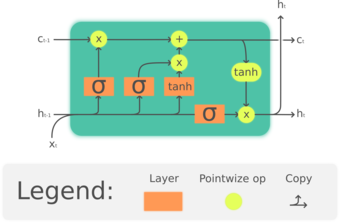
\includegraphics[scale=2.2]{lstm}
				\caption{Architettura di una LSTM}
			\end{center}
		\end{figure}		
		
		Come possiamo vedere dalla figura, una cella LSTM in realtà è formata da più strati diversi, 3 con attivazione a sigmoide e 1 con attivazione a tangente iperbolica.
		In particolare:
		\begin{itemize}
			\item lo strato più a sinistra è detto "\textit{forget gate}", e l'output regola la modifica del gradiente precedente;
			\item i due strati centrali sono detti "\textit{input gate}", quello attivato dalla sigmoide decide quali valori andranno aggiunti alla memoria della rete, mentre quello attivato dalla tangente iperbolica dà in output i nuovi valori che potrebbero essere aggiunti. La moltiplicazione \textit{point-wise} successiva darà il vettore di valori che saranno aggiunti alla memoria; 
			\item lo strato più a destra è detto "\textit{output gate}", e modifica l'output finale della rete.
		\end{itemize}
		
		\subsection{Architettura del Modello}
			Il modello di \textit{deep learning} implementato è formato da 5 strati, di cui 2 che sono LSTM:
			\begin{enumerate}
				\item un primo strato \verb|Masking|;
				\item due strati \verb|LSTM|;
				\item uno strato \verb|Dropout|;
				\item uno strato finale \verb|Dense|.
			\end{enumerate}
			
				\subsubsection{Masking}
					Lo strato \verb|Masking| ha come obiettivo quello di eliminare il padding, in modo da rendere meno costoso il learning.
					
				\subsubsection{LSTM}
					I due strati \verb|LSTM| sono consecutivi, il primo ha l'opzione \verb|return_sequences| attivata, in modo da dare in output allo strato successivo tutti i vettori della sequenza, e non solo l'ultimo. Inizialmente utilizzavamo soltanto uno strato \verb|LSTM|, tuttavia abbiamo osservato che questa versione con due strati offre performance migliori.; inoltre, l'aggiunta del secondo strato, ci ha permesso anche di poter avere uno strato che restituisse in output tutta la sequenza elaborata, in modo da poterla analizzare in un altro strato \verb|LSTM|.
					
				\subsubsection{Dropout}
					Lo strato \verb|Dropout| modifica alcuni input in modo casuale settandoli a $ 0 $, per tentare di prevenire l'\textit{overfitting}. La probabilità di impostare un input a $ 0 $ è $ 0.5 $.
					
				\subsubsection{Dense}
					Lo strato \verb|Dense| ha come scopo quello di restituire la classificazione finale, usando come funzione di attivazione la sigmoide. 
			
	
			\begin{figure*}
				\begin{center}
					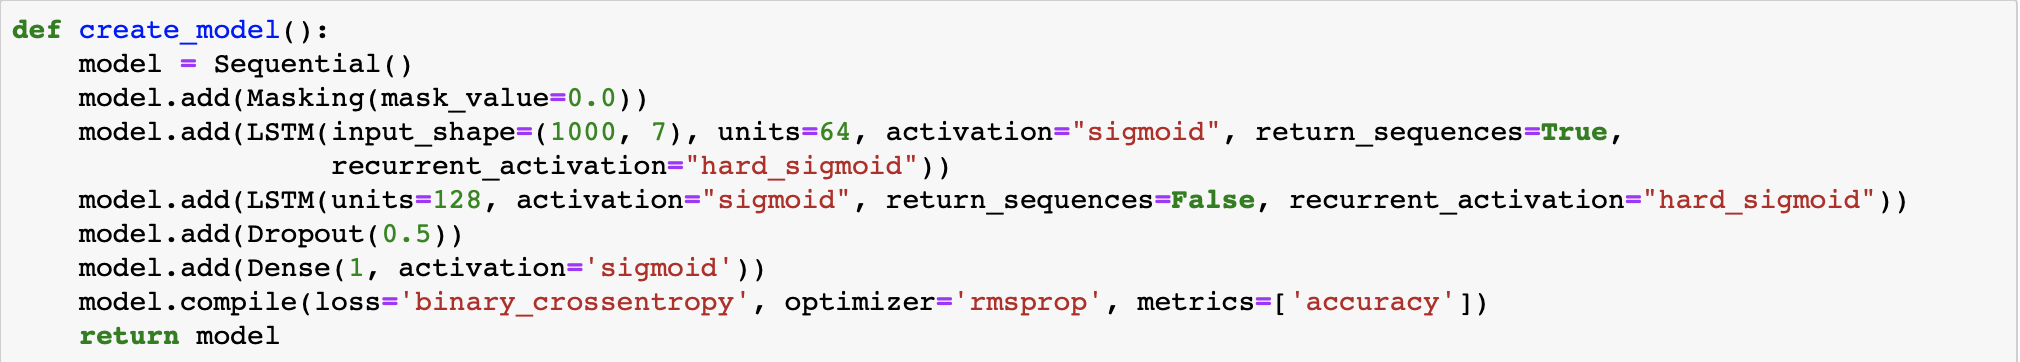
\includegraphics[scale=.45]{def_model}
					\caption{Definizione del modello}
				\end{center}
			\end{figure*}					
					
			\begin{figure*}
				\begin{center}
					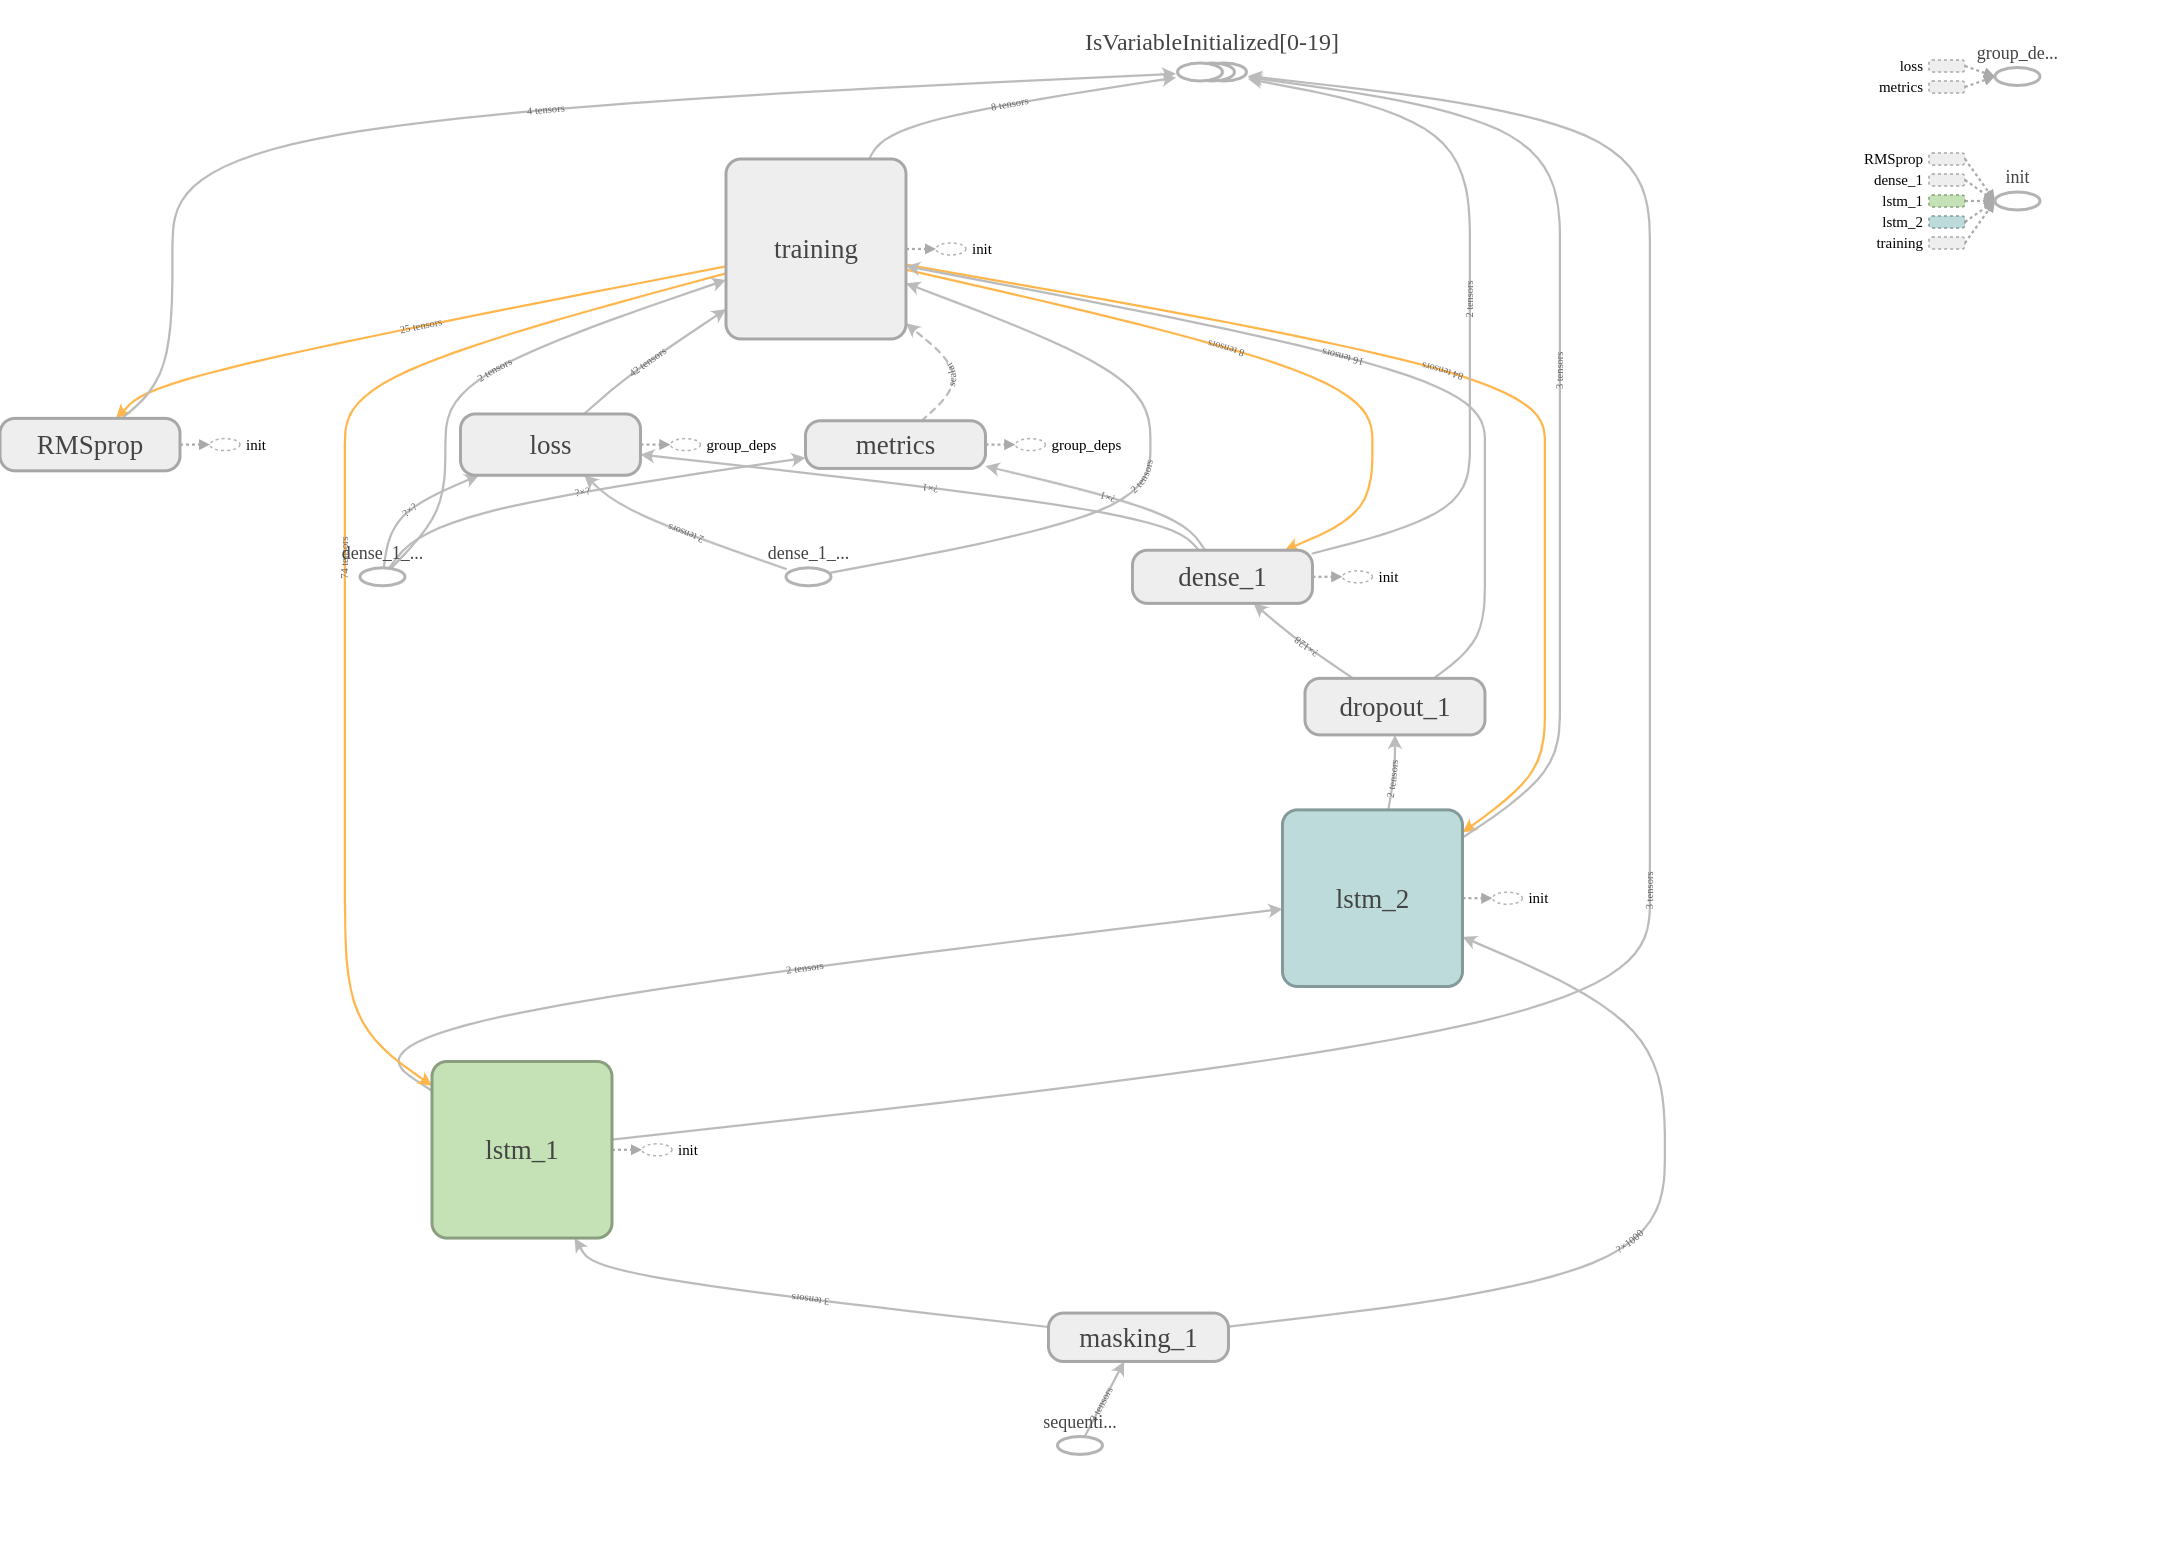
\includegraphics[scale=.23]{lstm_model}
					\caption{Modello durante la fase di training, rappresentazione da TensorFlow}
				\end{center}
			\end{figure*}		
		


\chapter{Training e Test}
	Il dataset raccolto contiene parole scritte da 23 persone diverse, per un totale di 845 sample. La parola scelta da far scrivere agli utenti è "Computer", in corsivo. \\
	Sia il training che i vari test sono stati eseguiti su un computer fisico con le seguenti specifiche:
	\begin{itemize}
		\item CPU: Intel Core i7 8700K;
		\item GPU: NVIDIA GeForce GTX 1070;
		\item RAM: 32 GB @ 3200 MHz.
	\end{itemize}
	
	\subsubsection*{Docker}
	Al fine di poter sfruttare la potenza calcolatrice della GPU abbiamo utilizzato il sistema Docker. Docker è un sistema di virtualizzazione che permette di creare delle macchine virtuali, detti "\textit{container}", che condividono il kernel (in modo da offrire prestazioni migliori rispetto ad una semplice macchina virtuale). Quel che abbiamo fatto è stato creare un container al cui interno viene eseguito un Jupyter Notebook. Inoltre, ci ha permesso anche di facilitare il deploy, rendendolo possibile su qualsiasi macchina (poiché i Jupyter Notebook possono essere eseguiti in remoto) e fornendo anche maggior protezione da eventuali attacchi informatici (in quanto il programma viene eseguito all'interno di una macchina virtuale). 
	
	\section{Training}
		È stato effettuato un training apposito per riconoscere alcuni degli utenti che sono stati registrati, generandone i relativi modelli. \\ 
		Ogni training ha previsto 110 \textit{epochs}, con un \textit{batch} di 32 elementi; inoltre è stata effettuata, in ogni \textit{epoch}, una fase di \textit{validation} usando un terzo delle parole presenti nell'insieme di training. \\
		Chiaramente, il dataset risulta ancora abbastanza contenuto, quindi i dati che saranno presentati nella successiva sezione non sono indicativi delle reali performance del sistema, per adesso. Nonostante ciò, ha senso analizzarli per avere una prima impressione dei modelli sviluppati.
		
	\section{Test}
		
		\subsection{DTW}
			Per quanto riguarda il DTW abbiamo potuto effettuare un numero limitato di test, soprattutto per problemi di tempo. Poiché Python non supporta esecuzioni in multithread, il programma è stato eseguito su un singolo processore, rendendolo purtroppo più lento. \\
			Nonostante ciò, abbiamo ottenuto alcuni risultati abbastanza promettenti:
				\begin{figure}[H]
					\begin{center}
						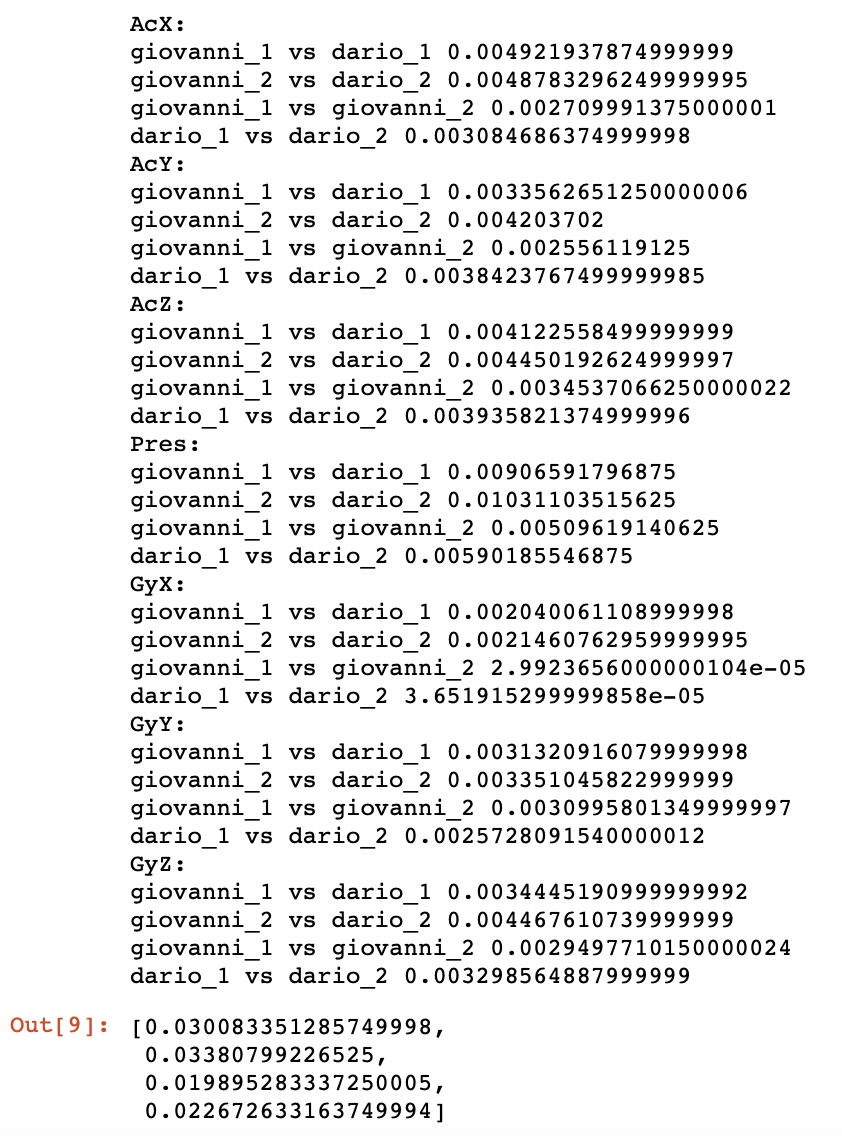
\includegraphics[scale=.25]{dtw_test}
						\caption{Risultati del test del DTW su due coppie di parole di due utenti registrati}
					\end{center}
				\end{figure}	
				
			Per ogni test del DTW (questo è solo uno di quelli che abbiamo fatto) consideriamo due parole per ogni utente e le confrontiamo con altre due parole di un altro utente. Per ogni componente (accelerometro, pressione, giroscopio) stampiamo in output le distanze per ogni combinazione fra le quattro parole; infine, stampiamo un array che contiene la somma delle rispettive distanze per ognuna delle quattro coppie di parole. \\
			Idealmente, le coppie composte da parole di due utenti diversi dovrebbero avere una somma delle distanze maggiore rispetto alla somma di distanze di coppie di parole dello stesso utente. Ciò che abbiamo potuto osservare, limitatamente ai pochi test che abbiamo effettuato, è che quest'assunzione sembra essere vera in tutti i casi. \\
			In un secondo tipo di test, che abbiamo potuto effettuare un'unica volta in quanto troppo lento (l'esecuzione è durata fra le 6 e le 7 ore),  abbiamo selezionato casualmente una parola dal dataset ed abbiamo calcolato la distanza $ d $ (come media delle distanze di ognuna delle 7 componenti) di tutte le parole del dataset da essa. Il test ha avuto un esito molto positivo, generando una curva ROC la cui AUC è molto vicina a 1:
			
			\begin{figure}[H]
				\begin{center}
					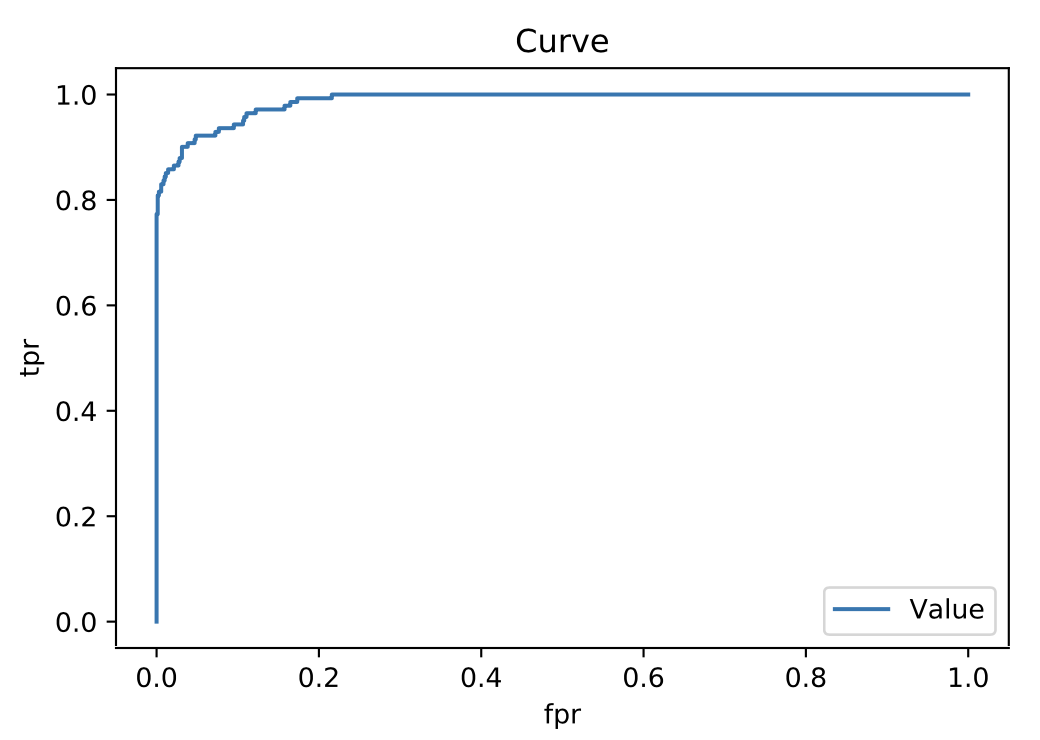
\includegraphics[scale=.4]{ROC_DTW}
					\caption{Curva ROC ottenuta considerando la "vicinanza" ($ 1 - d $); AUC $ \cong 0.99 $}
				\end{center}
			\end{figure}
			
			Visto che le feature sono state scalate fra $ 0 $ e $ 1 $, la distanza massima è proprio $ 1 $, e di conseguenza la vicinanza è data come la differenza fra $ 1 $ e la distanza calcolata. 
			
			\begin{figure}[H]
				\begin{center}
					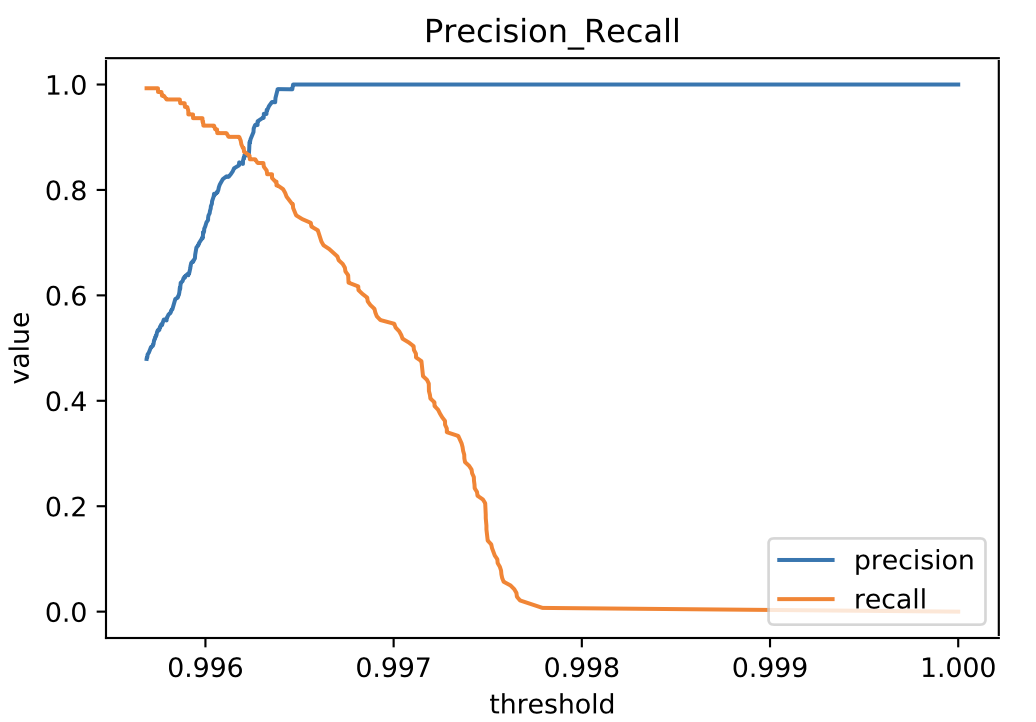
\includegraphics[scale=.6]{precision_recall_DTW}
					\caption{Curve di \textit{precision} e \textit{recall} al variare della threshold}
				\end{center}
			\end{figure}
			
			\begin{figure}[H]
				\begin{center}
					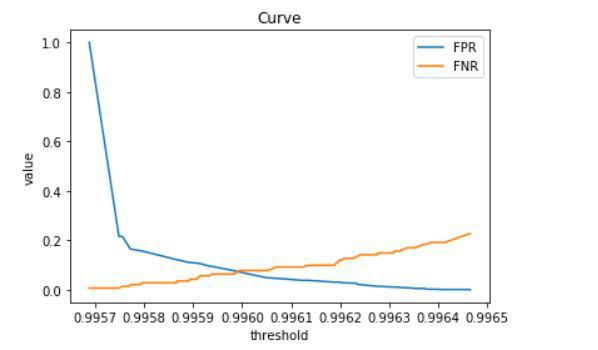
\includegraphics[scale=.6]{fpr_fnr_DTW}
					\caption{Curve di FPR e FNR al variare della threshold, si noti che l'EER è poco meno di $ 0.996 $, con i due rate che sono meno di $ 0.1 $}
				\end{center}
			\end{figure}
		
		\newpage		
		
		\subsection{LSTM}
		
			Il modello basato sulle LSTM ha raggiunto ottime prestazioni in poche epoch di training, tenendo comunque in considerazione che il dataset è relativamente piccolo. Includiamo solo uno dei modelli che abbiamo allenato ed i relativi test effettuati, in quanto altri esempi risulterebbero ridondanti. 
			\begin{figure}[H]
				\begin{center}
					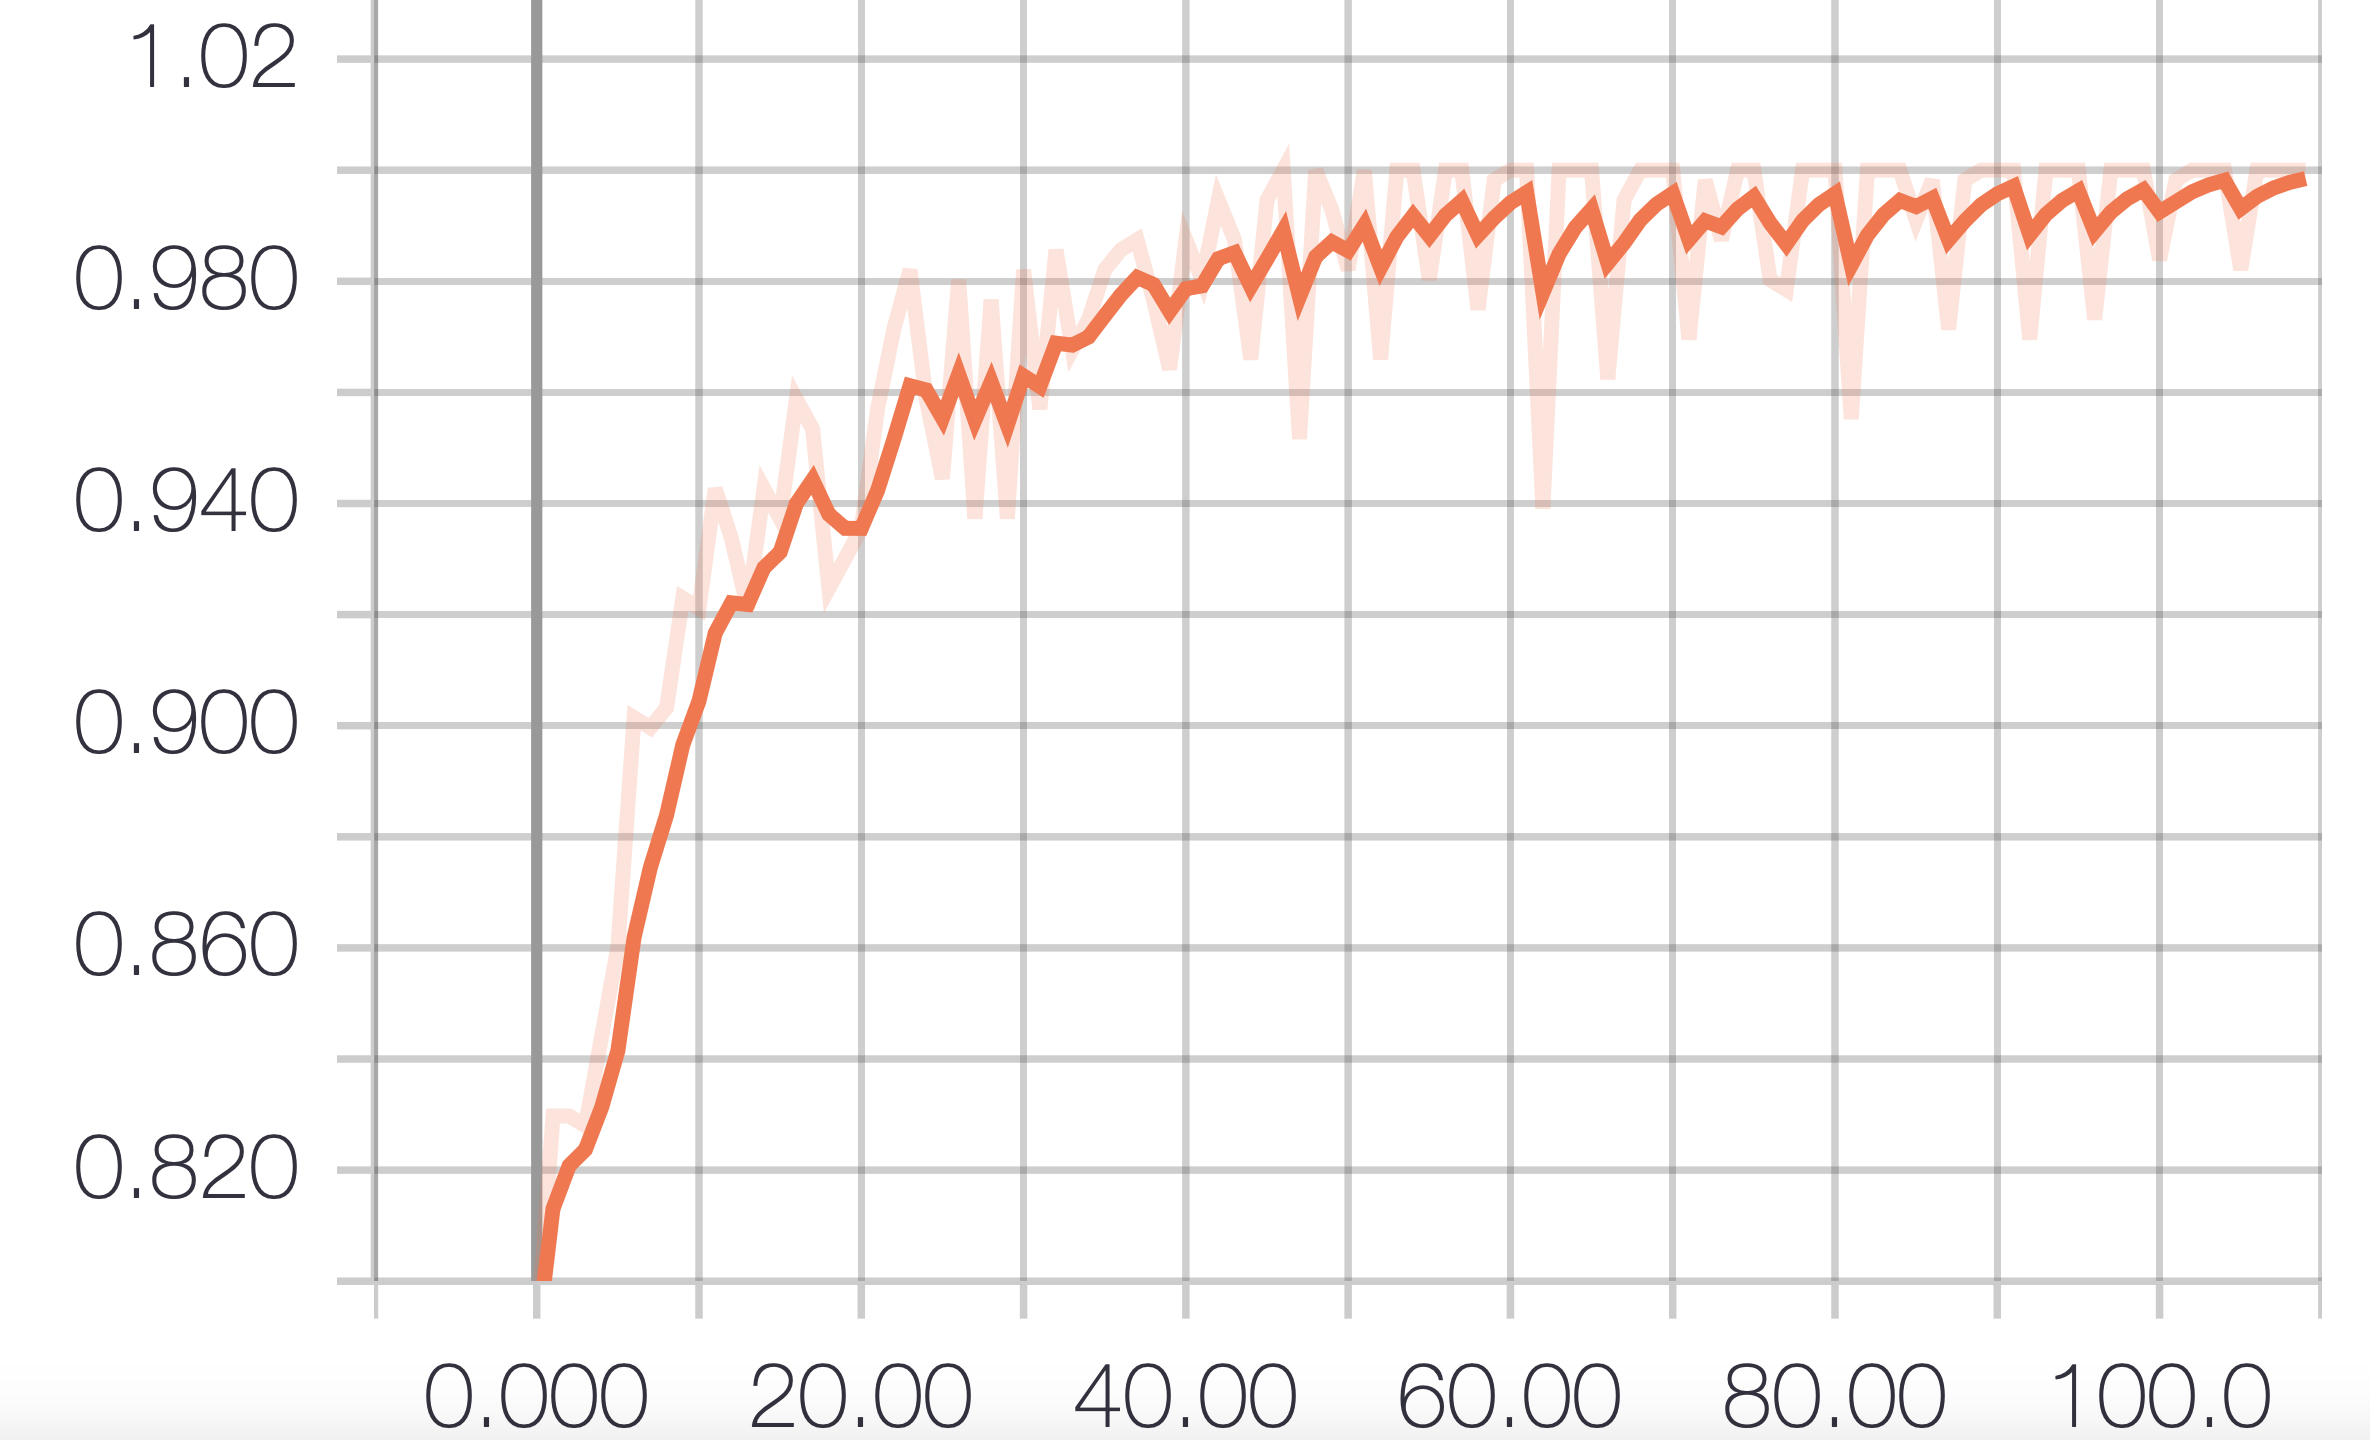
\includegraphics[scale=.175]{acc_Antonio}
					\caption{Accuracy del modello sul training set}
				\end{center}
			\end{figure}
			
			\begin{figure}[H]
				\begin{center}
					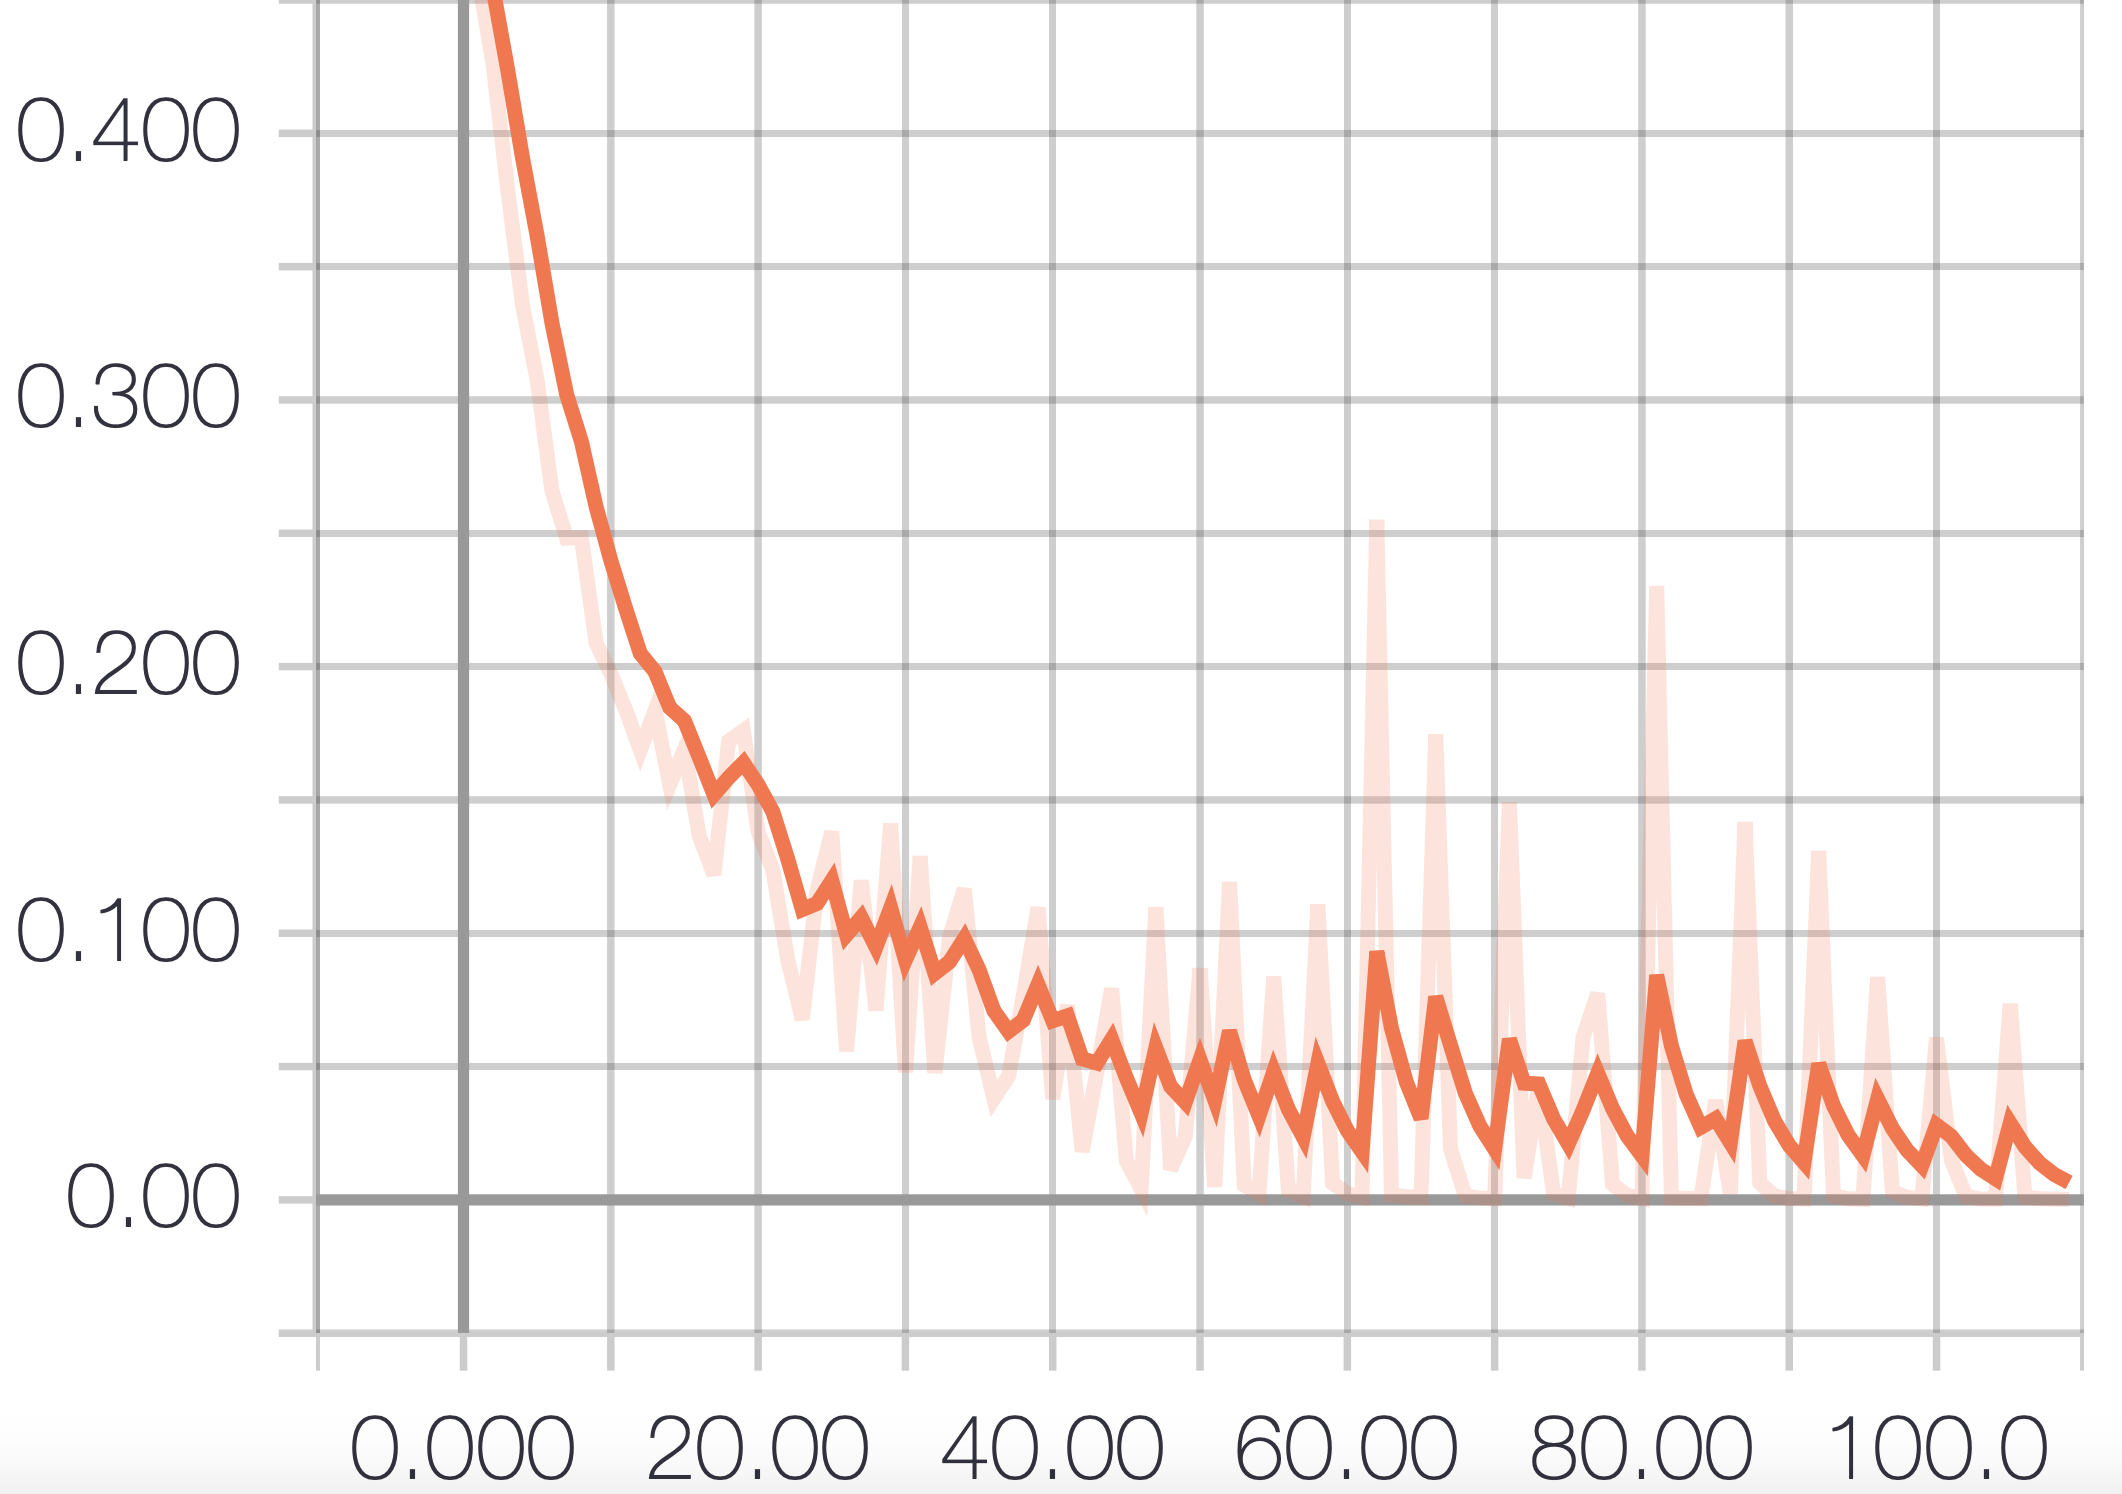
\includegraphics[scale=.175]{loss_Antonio}
					\caption{Loss del modello sul training set}
				\end{center}
			\end{figure}
			
			\begin{figure}[H]
				\begin{center}
					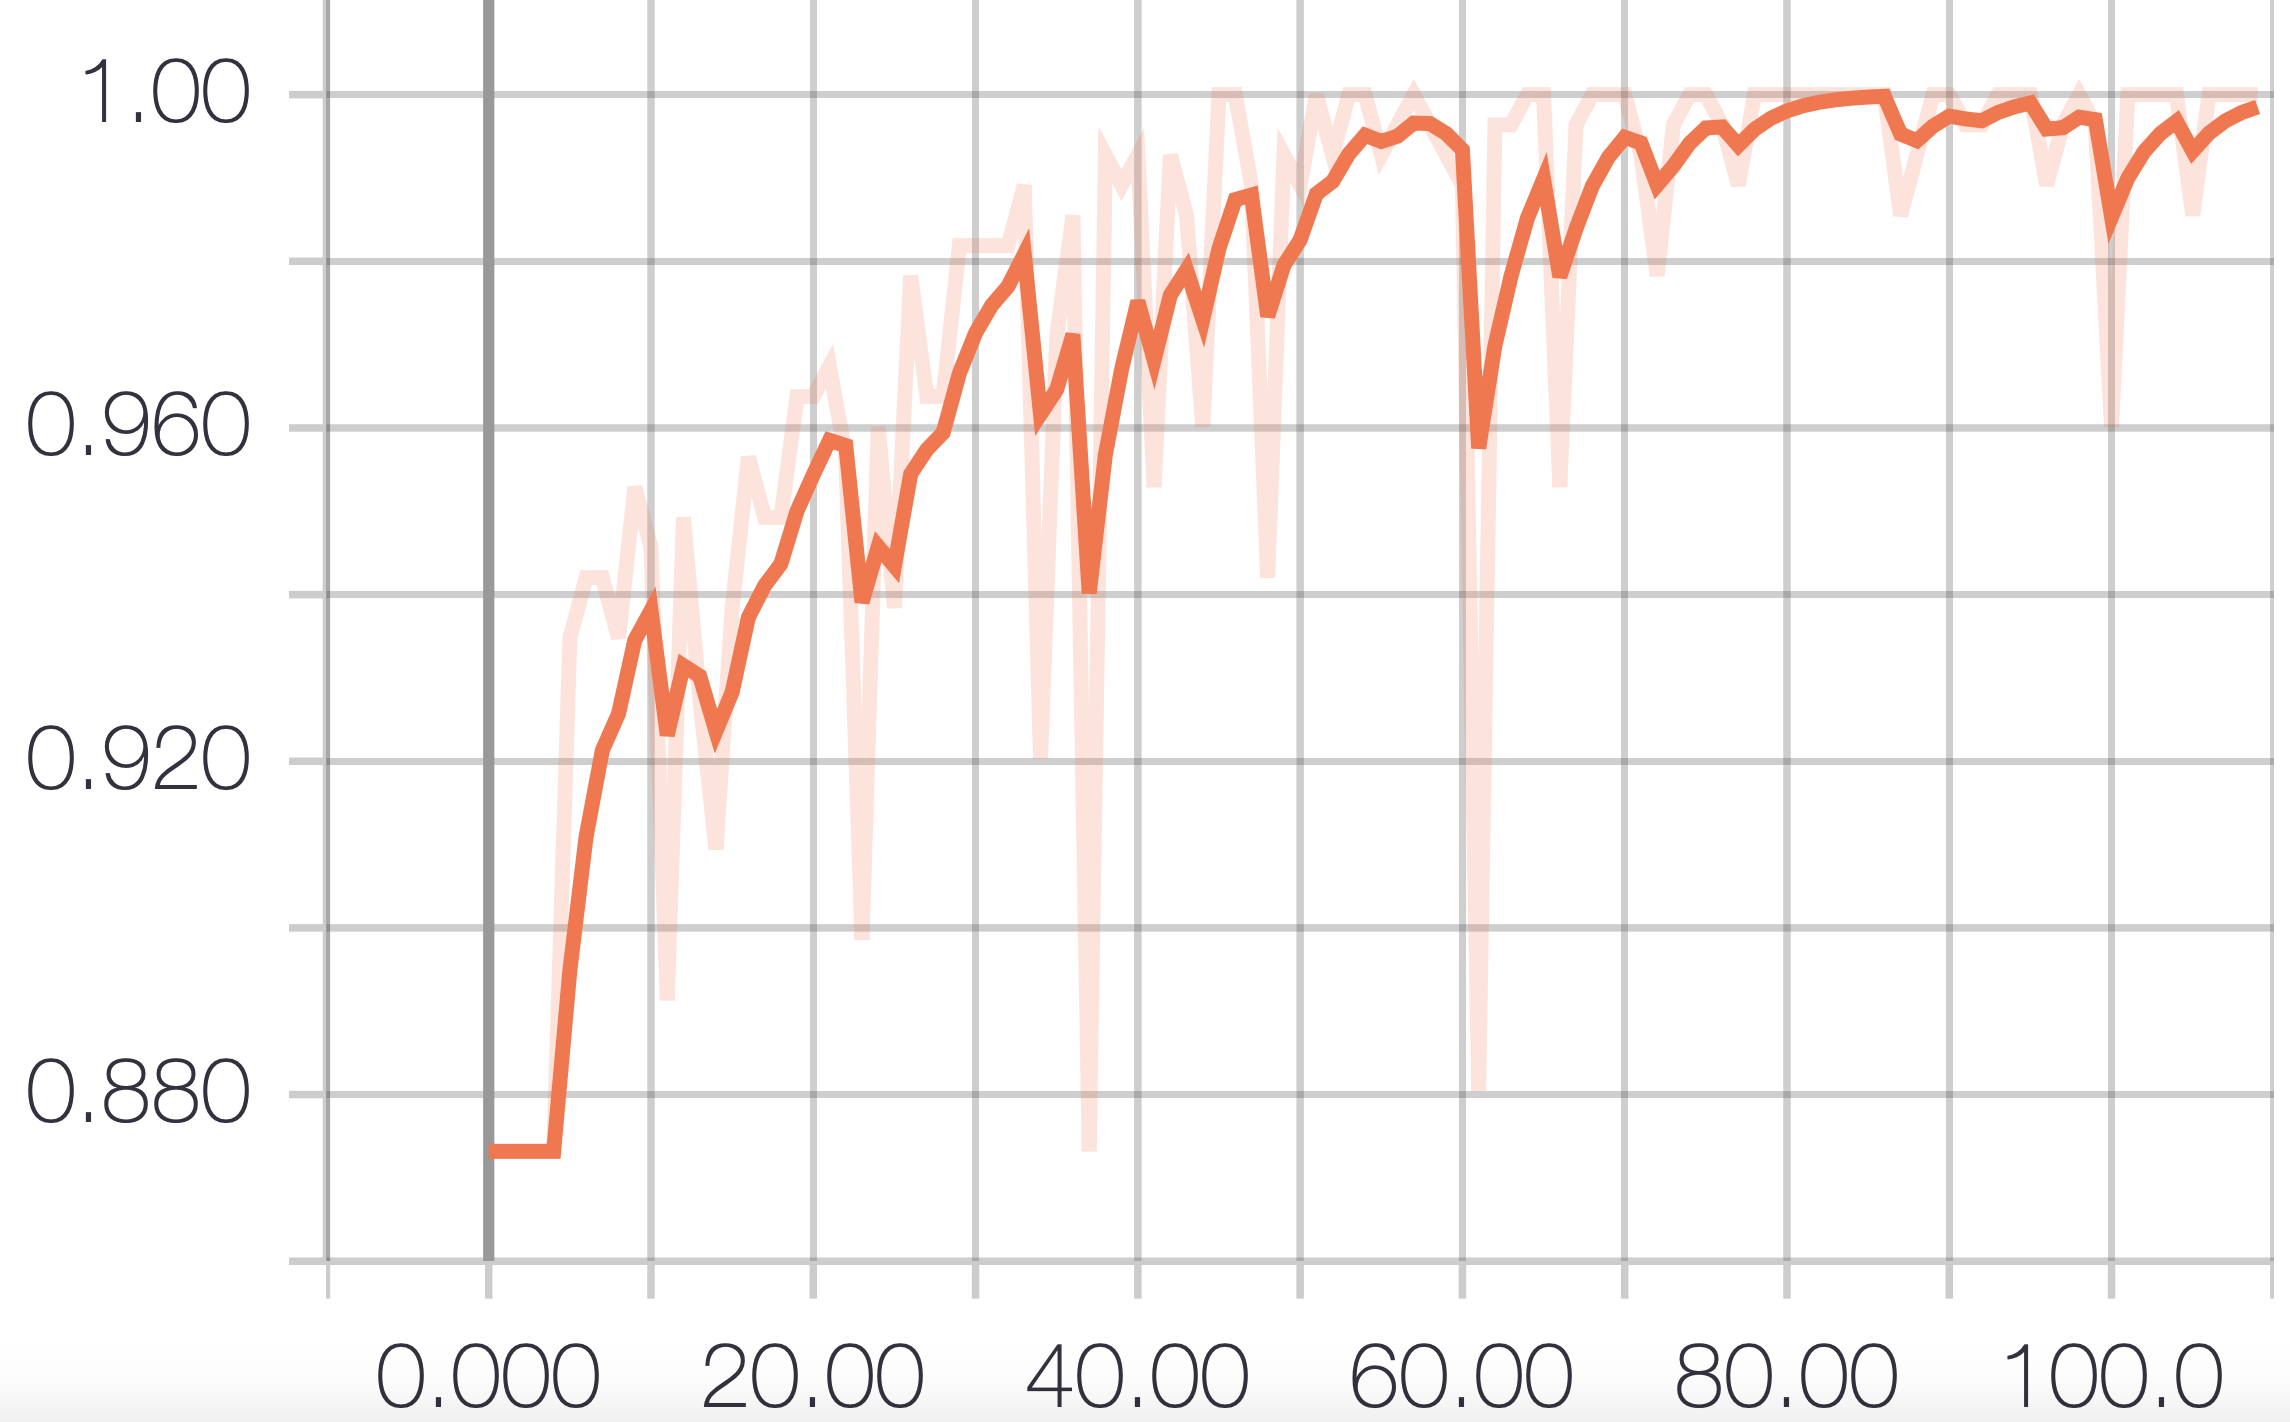
\includegraphics[scale=.175]{val_acc_Antonio}
					\caption{Accuracy del modello sul validation set}
				\end{center}
			\end{figure}
			
			\begin{figure}[H]
				\begin{center}
					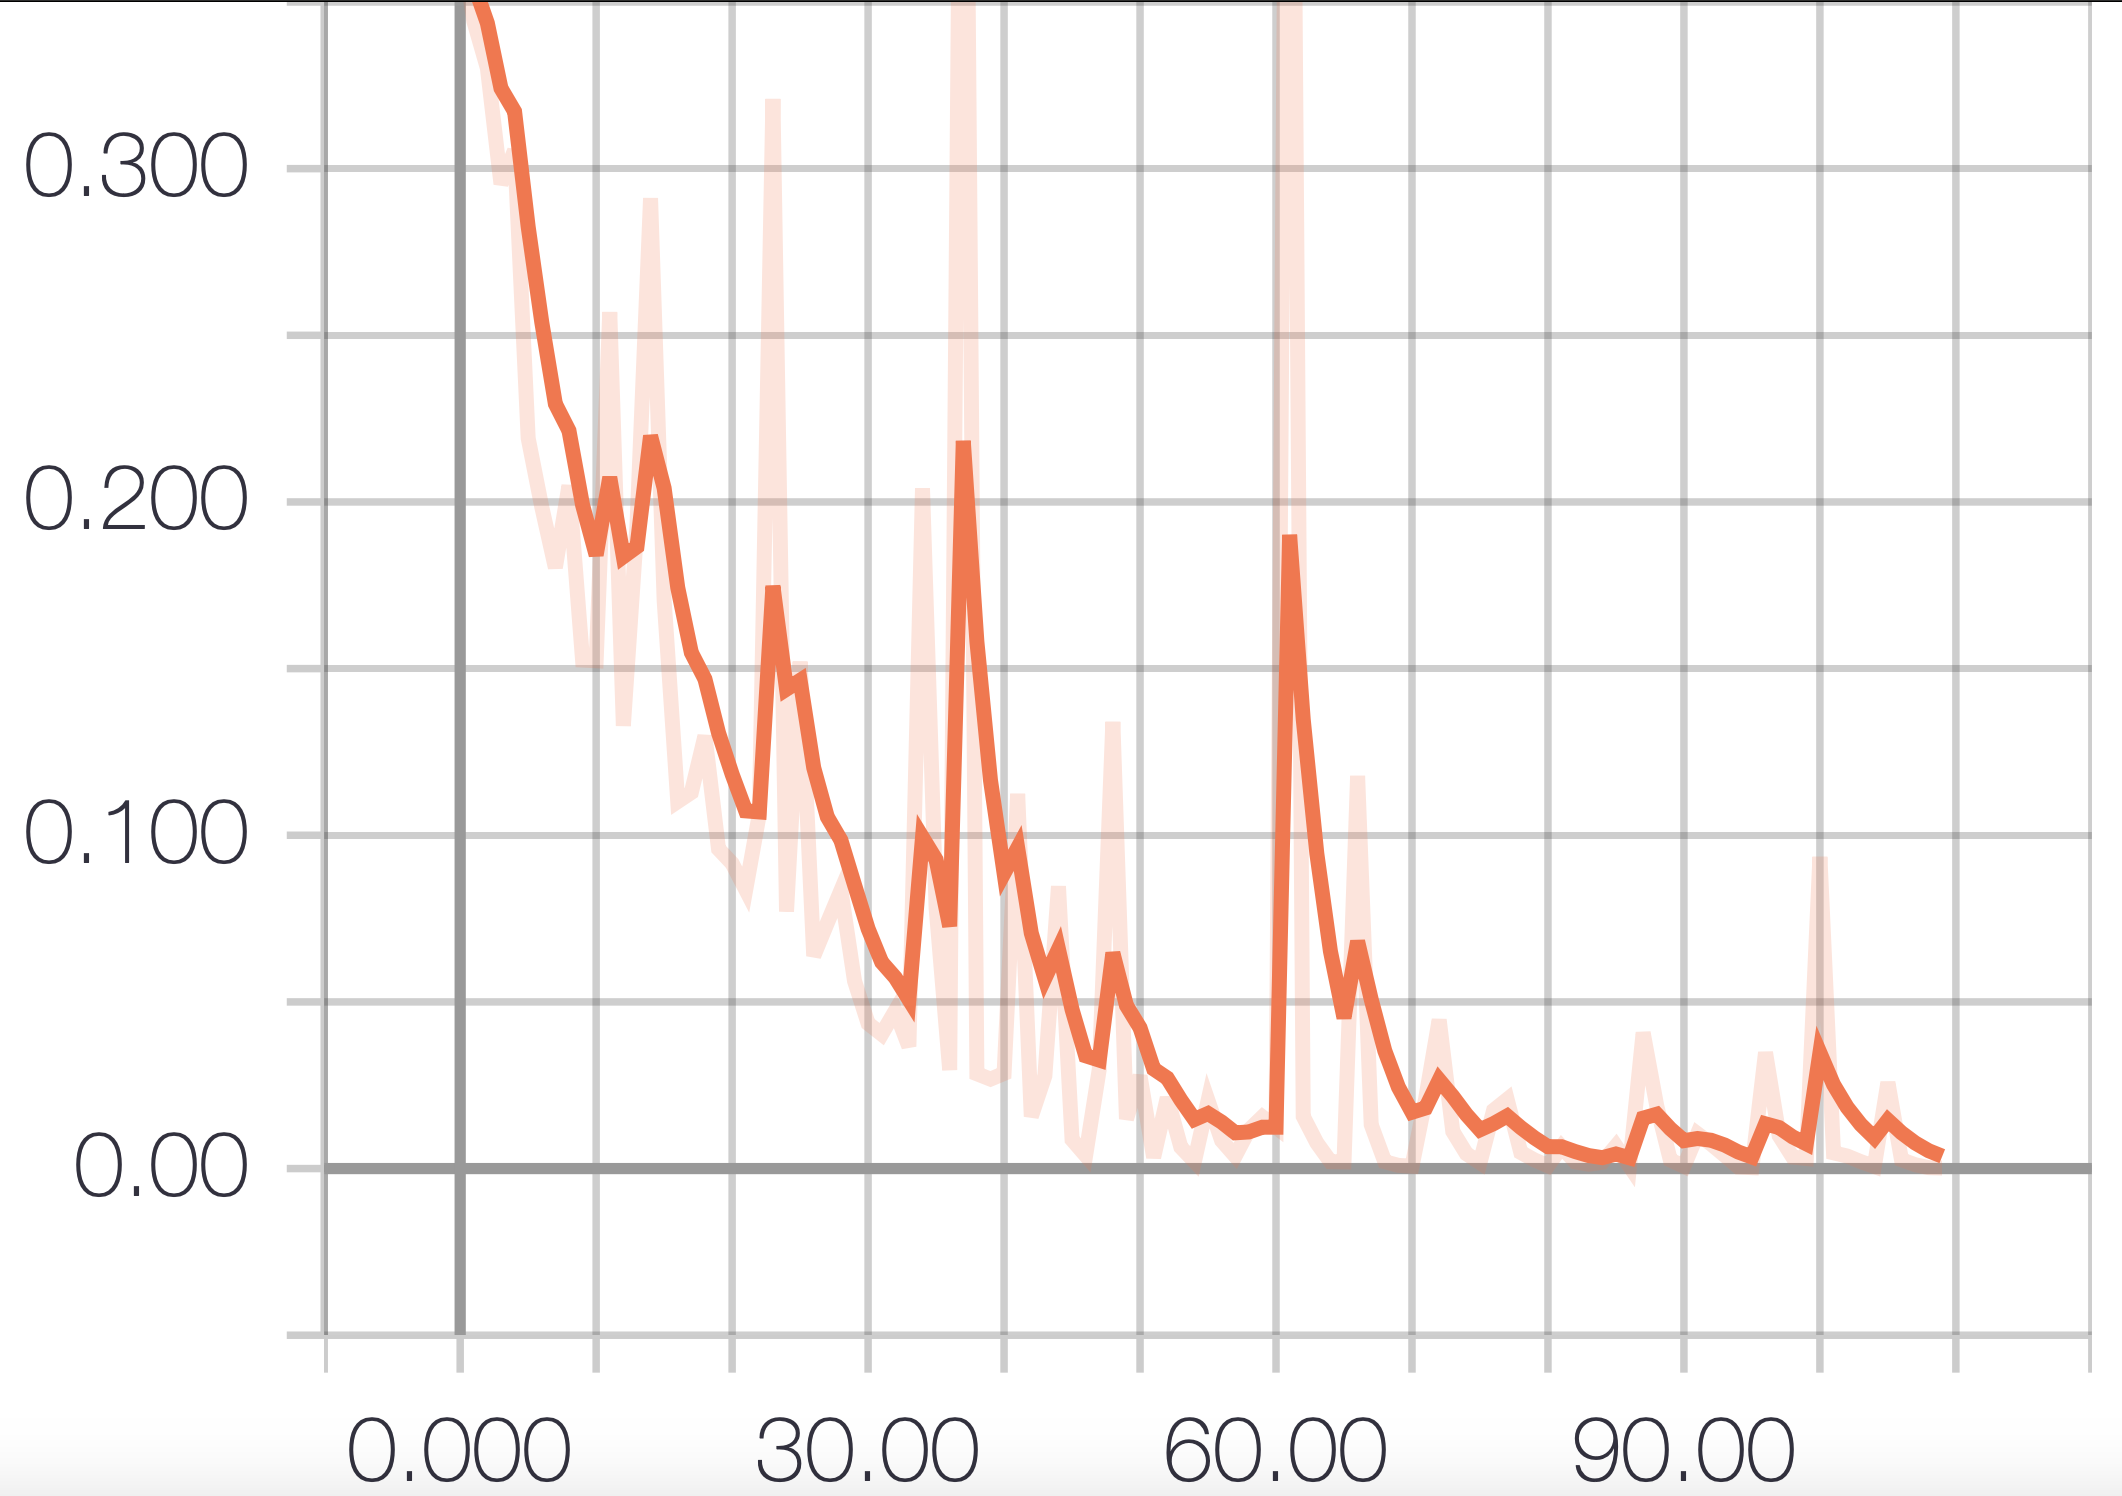
\includegraphics[scale=.175]{val_loss_Antonio}
					\caption{Loss del modello sul validation set}
				\end{center}
			\end{figure}
			
			\begin{figure*}
				\begin{center}
					\label{figure:prediction}
					\includegraphics[scale=.5]{test_Antonio}
					\caption{Predizioni del modello su parole scritte in un altro momento rispetto a quelle usate nel training}
				\end{center}
			\end{figure*}
			\newpage
			\begin{figure}[H]
				\begin{center}
					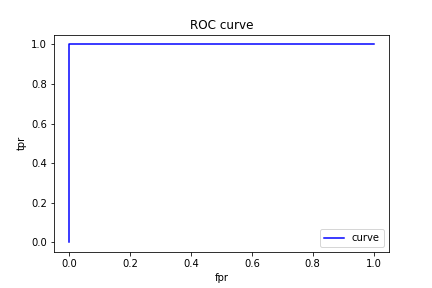
\includegraphics[scale=.5]{ROC_Antonio}
					\caption{Curva ROC del modello allenato}
				\end{center}
			\end{figure}
			
			\begin{figure}[H]
				\begin{center}
					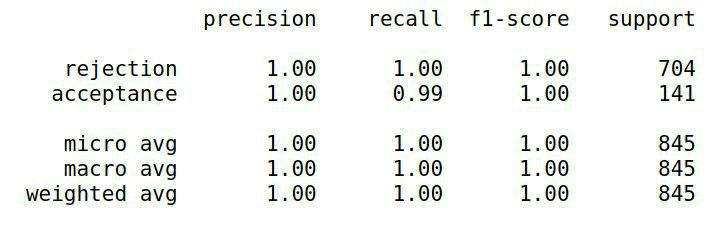
\includegraphics[scale=.4]{measures_table_LSTM}
					\caption{Report delle statistiche del modello}
				\end{center}
			\end{figure}
			\newpage
			Particolarmente interessante è la figura sulle predizioni, che in sostanza rappresenta il task principale della PeterPen, ossia riconoscere una persona dai dati che si raccolgono mentre scrive, sfruttando un modello allenato su altri dati dello stesso utente ma ottenuti in un momento precedente. Dai test che abbiamo effettuato sembra che il modello riesca effettivamente a riconoscere l'utente, con un accuracy di quasi il 99\%. \\
			Il modello inoltre non sembra essere afflitto da problemi di \textit{overfit} o \textit{underfit}, in quanto raggiunge accuracy molto simili nelle ultime epoche per il training set ed il validation set, oltre al 99\% di accuracy sul nuovo set di parole come scritto sopra. \\


\chapter{Lavori futuri}

	Innanzitutto, vorremmo effettuare una stampa della scocca più precisa. Abbiamo incontrato varie difficoltà nel montare la penna, dovute principalmente alle imprecisioni della stampante. \\
	Inoltre, andrebbe sviluppato anche un chip dedicato, in quanto la maggior parte dei pin sull'ESP8266 è inutilizzato. \\
	Per quanto riguarda il lato software, ci sono due possibili sviluppi. 
	\\ Dal lato DTW, si potrebbe provare a dare dei pesi alle singole feature nel calcolo del costo. Questa possibile modifica nasce dall'osservazione che, con molta probabilità, nel calcolo della distanza fra due parole scritte, ci sono alcune componenti dei dati che potrebbero essere più importanti di altre. Inoltre, vanno necessariamente fatti più test, per poter verificare in modo più attendibile le prestazioni.
	\\ Infine, abbiamo osservato che il modello di deep learning, allenato soltanto per riconoscere la parola "Computer" scritta da un solo utente, ha "erroneamente" riconosciuto anche dei "Ciao" \\ scritti dallo stesso utente. Questo ci fa pensare che, con alte probabilità, il modello si potrebbe prestare anche al riconoscimento della scrittura dell'utente, allenandolo su varie parole diverse scritte dallo stesso.
	
	\begin{figure}[H]
		\begin{center}
			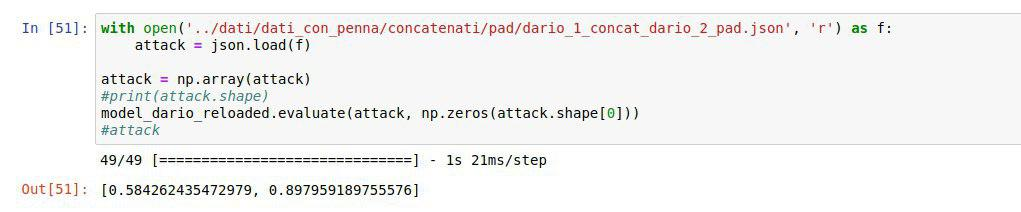
\includegraphics[scale=.3]{scrittura_dario}
			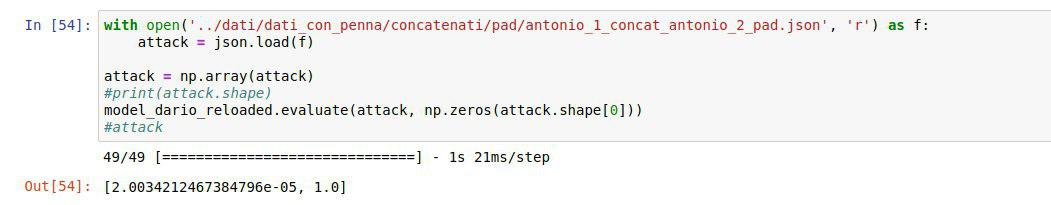
\includegraphics[scale=.3]{scrittura_antonio}
			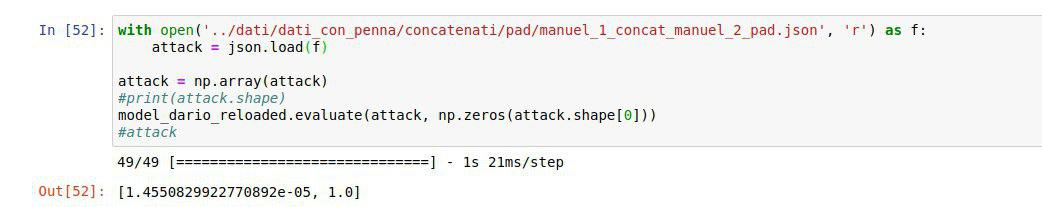
\includegraphics[scale=.3]{scrittura_manuel}
			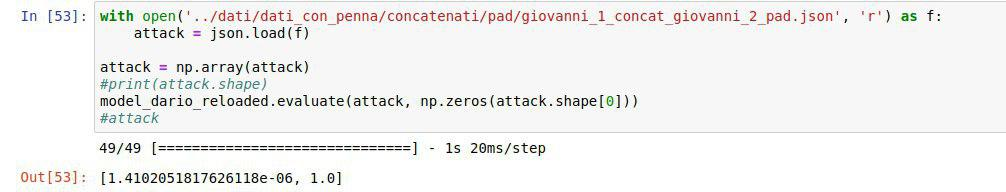
\includegraphics[scale=.3]{scrittura_giovanni}
			\caption{ Come si può osservare, il modello rifiuta (correttamente) gli impostori, mentre circa nel 10\% dei casi riesce a riconoscere correttamente l'utente, nonostante non abbia mai visto quella sua  parola}
		\end{center}
	\end{figure}



\bibliographystyle{myIEEEtranS}
\bibliography{mybib}{}

\end{document}